%% Use this line for the final version of your report
\documentclass[final,american]{include/RaM/RaM-MScReport}

%% Use this line for the draft versions of your report, it enables rro/notes/line numbers/date in footer
%\documentclass[lineno,UKenglish]{include/RaM/RaM-MScReport}

\settitle{Comparing processing techniques for real-time force estimation from sEMG}
\setauthor{Tjeerd Bakker}
%-------------------------------------------------------------------------------------------------
% This settings.tex contains settings required for *all* documents (reports, presentations, etc)
% Project or Report specific settings should go to their own settings files (eg CE/settings.tex)
% This file is included after the class definition and before project and report specific settings 
%-------------------------------------------------------------------------------------------------

%--------Useful packages (required by the example files, turn off if you do not use them)-------
\usepackage{babel}					% Add language specific support
%\usepackage{makeidx}				% Index support
%\usepackage[totoc,justific=RaggedRight]{idxlayout}	% Make last page of index balanced and add index to toc
\usepackage{caption}				% Provides means to style captions

\DeclareCaptionType{equ}[][]
%\captionsetup[equ]{labelformat=empty}

%\usepackage{subcaption}				% Provides support for (sub)figures and (sub)tables
%\usepackage{float}					% Improved interface for floating objects (eg figures, tables, ...)
\usepackage{enumitem}				% Add styling support to (enumerate) environments
\usepackage{listings}				% Allows (external) source files to be shown in a syntax highlighted way
\usepackage{amsmath}				% Provides miscellaneous enhancements for documents containing formulas
\usepackage{datetime}				% Provides commands for displaying the current time
%\usepackage{etoolbox}				% Provides \AtBeginEnvironment command
\usepackage{eurosym}				% Defines \euro command to display euro symbols
\usepackage{siunitx}
\usepackage{hyperref}
\usepackage{float}


%\usepackage{appendix}				% Makes it possible to modify appendix numbering
%\usepackage{longtable}				% Allows tables to span multiple pages
%\usepackage{units}					% Shows units (eg m/s) in a nice way
%\usepackage{ctable}				% Provides \ctable command for the typesetting of table and figure floats
%\usepackage{ccaption}				% Support continuation captions (eg multi-page tables)
%\usepackage{verbatim}				% Adds verbatim environment, in which texts are exactly copied to the output
%\usepackage{pdfpages}				% Include PDF pages/documents in the current document
\usepackage{include/files/requirements}

\iffinalversion
	\usepackage[final]{include/files/notes}% Add note commands, [final] removes all notes from the document
	\usepackage[final]{include/files/rro}  % Add Rich Report Outline support, [final] removes all RRO output from document
\else
	\usepackage{include/files/notes}       % Add note commands
	\usepackage{include/files/rro}         % Add Rich Report Outline support
\fi

% Add wrongly (or unknown) hyphened words here (space separated and - at possible hyphenation positions):
%\hyphenation{}

%% Spacing possibilities for captions are available as well
% See captions.pdf for all options!
\captionsetup{font=small,labelfont=bf}

%% Center all figures by default
%% http://tex.stackexchange.com/questions/2651/should-i-use-center-or-centering-for-figures-and-tables
\makeatletter
\g@addto@macro\@floatboxreset\centering
\makeatother

%% Make use small font size in verbatim environment
% Note: AtBeginEnvironment is provided by etoolbox package
%\AtBeginEnvironment{verbatim}{\small}

%% Include verbatim in the subfigure env
% From: subfig.pdf, section 4.4
% <Uncomment if verbatim is required in subfloat>:
%\makeatletter
%\newbox\sf@box
%\let\orig@subfloat\subfloat
%\renewenvironment{subfloat}[2][]%
%{ \def\sf@one{#1}%
%  \def\sf@two{#2}%
%  \setbox\sf@box\hbox
%  \bgroup}%
%{ \egroup
%  \ifx\@empty\sf@two\@empty\relax
%    \def\sf@two{\@empty}
%  \fi
%  \ifx\@empty\sf@one\@empty\relax
%    \orig@subfloat[\sf@two]{\box\sf@box}%
%  \else
%    \orig@subfloat[\sf@one][\sf@two]{\box\sf@box}%
%  \fi}
%\makeatother
%% Uncomment till here
  
%% Automatically provide H option for floats
% Requires float package
% \floatplacement{figure}{H} 
% \floatplacement{table}{H} 

%% abbreviation making
\newcommand{\abbr}[1]{(\textit{#1})}

%%lstlisting settings
\lstset{	%aboveskip=20pt,%
		numbers=none, %no line numbers
%		numbers=left, %show line numbers
		numberstyle=\tiny,%
		frame=single,%
		frameround={t}{t}{t}{t},%
		numbersep=5pt,%
%		language=C,% (default) code language in the document
		captionpos=b,%
		xleftmargin=2em,
		framexleftmargin=1.5em,
		xrightmargin=2em,
		framexrightmargin=1.5em,
		morecomment=[s][\itshape]{<}{>}, %also define <> as comment
		morecomment=[s][\itshape]{[}{]} %also define [] as comment
}

%lstinline with empty language definition
\lstdefinelanguage{empty}{}
\newcommand{\mylstinline}[1]{{\lstinline[language=empty]{#1}}}

% Default value of top separator (empty space) of lists
\setlist{topsep=4pt}

\bibliographystyle{IEEEtran}

%% Don't show warnings like: ``PDF inclusion: found PDF version <1.x>, but at most version <1.4> allowed
% Uncomment if you experience these kind of warnings 
%\ifpdf
%	\pdfminorversion=6 
%\fi

%%%%%%%%%%%%%%%%%%%%%%%%%%%%%%%%%%%%%%%%
% Macros for commenting and correcting.
%%%%%%%%%%%%%%%%%%%%%%%%%%%%%%%%%%%%%%%%
\usepackage{xcolor}															%Needed to have some colored text
\usepackage{soul}															% Strike out text using \textst{...}
\newcommand{\crgk}[1]{\noindent\textcolor{blue}{{#1}}} 							%Corrections	
\newcommand{\cmgk}[1]{\noindent\textcolor{blue}{\emph{GK:} #1}}  					%Comments
\newcommand{\rmgk}[1]{\noindent\textcolor{red}{{\textst{#1}}}} 						%Remove
\newcommand{\rpgk}[2]{\noindent\textcolor{red}{{\textst{#1 }}\textcolor{olive}{{#2}}}}  	%Replace
\newcommand{\gk}[1]{\noindent\textcolor{red}{#1~Please: reread, reconsider, rephrase!}}
\newcommand{\csgk}{\cmgk{Clumsy sentence, please rephrase.}}     					%Improve sentence
\newcommand{\itgk}{\cmgk{Illegible text in graph. Please improve.}}  					%Improve text in figure
\newcommand{\wngk}[1]{
\vspace{4mm}
\fbox{\begin{minipage}{0.90\columnwidth}\noindent\textcolor{red}{#1}\end{minipage}}
\vspace{4mm}
}



\begin{document}
% Numbered roman style

\frontmatter

% this is just a temporary front page. You will can get the final front page from Jolanda when you are close to finishing your report.

% Use \maketitle or the available PDF when it is released (for student reports)
%\maketitle

% Enter the name of the official RaM title page PDF between the brackets
% ! This method disables the option of using EPS files in your report.
% ! If EPS images are required, use LaTeX source instead of the PDF file
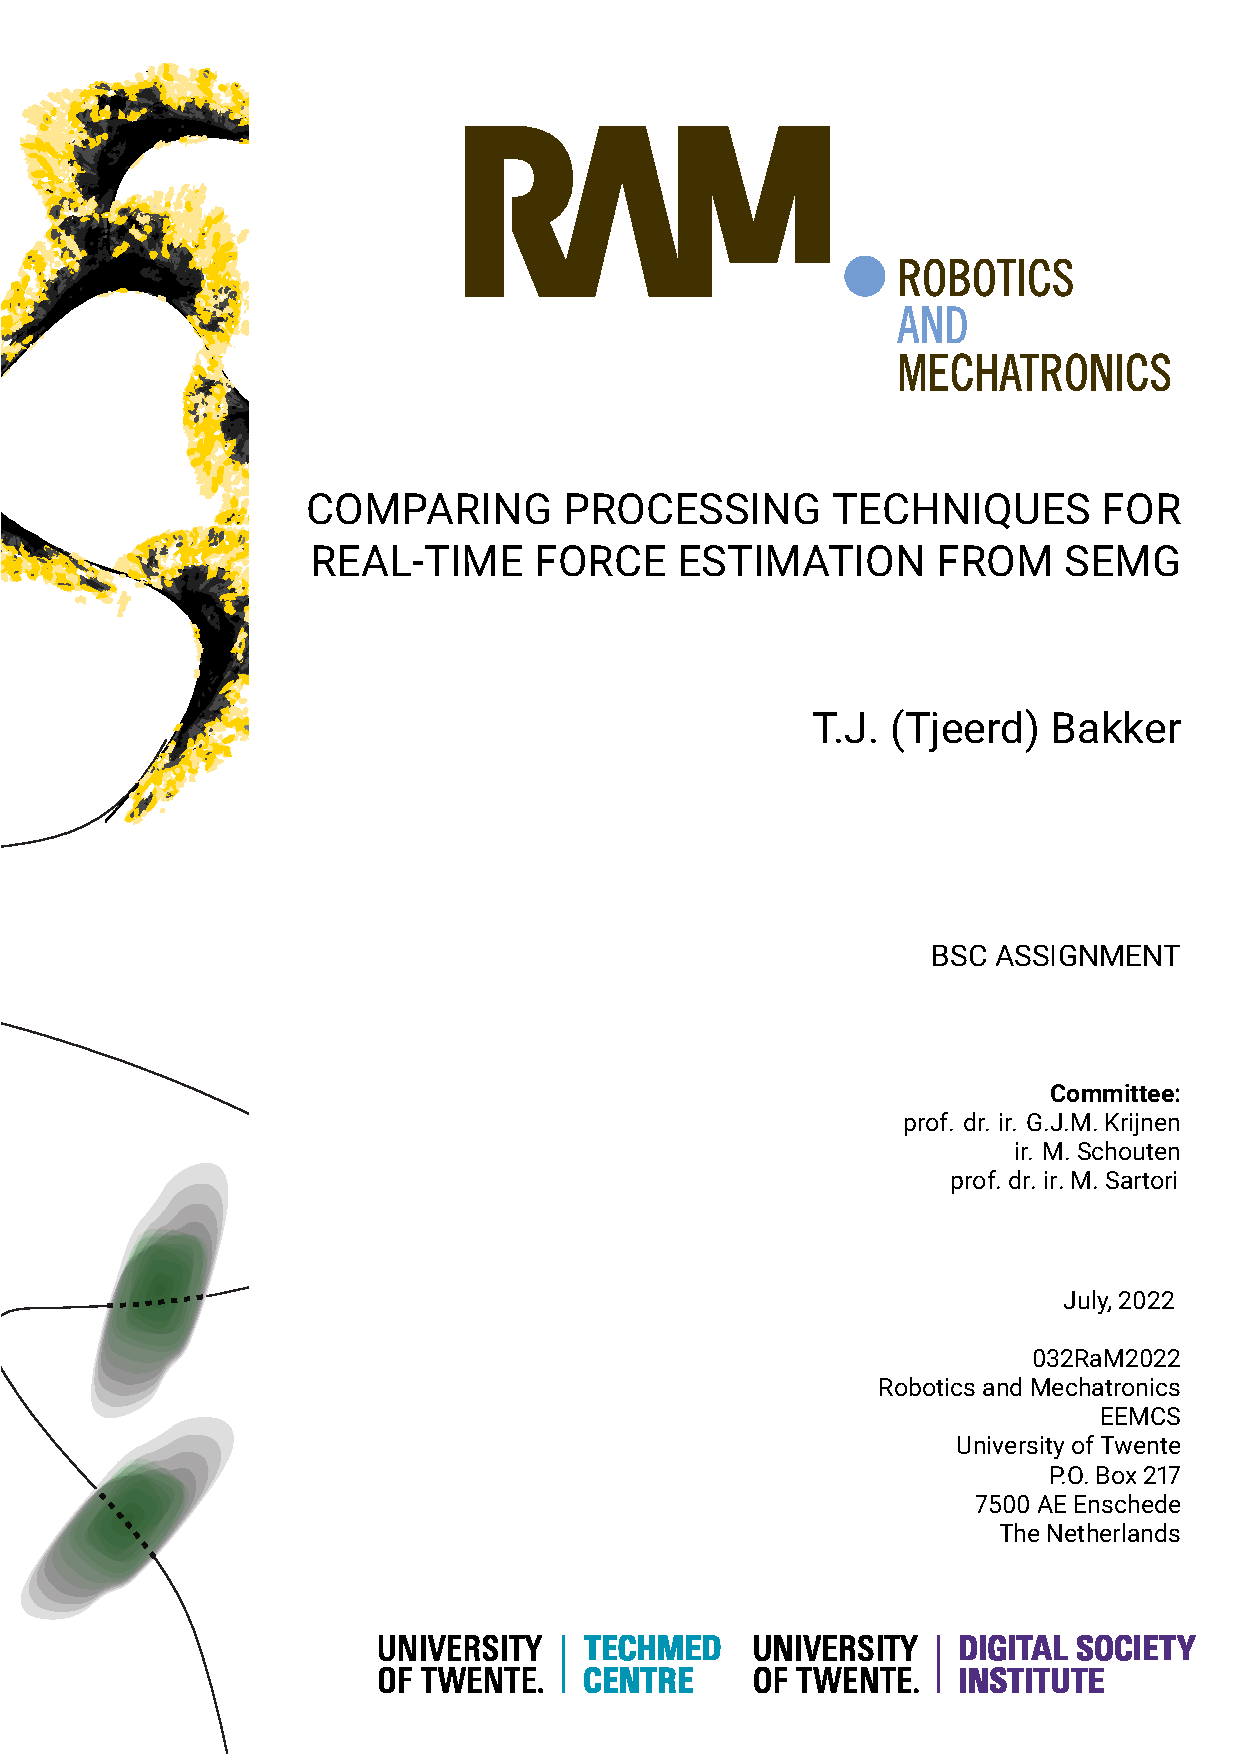
\includepdf{032bakker2022.pdf}


\cleardoublepage

\chapter*{Abstract}
\textcolor{brown}{
This bachelor thesis investigates to which extend adaptive filters can improve digital signal processing of surface Electromyography signals compared to standard static filters. < Insert more stuff once I finish the report > } \\

Provide a concise summary of the research conducted. Include the conclusions reached and the potential implications of those conclusions. Your abstract should also:

Consist of a single paragraph up to 250 words, with correct grammar and unambiguous terminology.
Be self-contained. No abbreviations, footnotes, references, or mathematical equations.
Highlight what is unique in your work.
Include 3-5 keywords or phrases that describe the research to help readers find your paper.

1. What did you do?
2. Why did you do it?
3. What did you find?
4. What do you conclude?

% Add the table of contents pages (TOC)
\tableofcontents

% The report starts here

\mainmatter

%\chapter*{Useful definitions}
\section{List of symbols}
This table contains an overview of the symbols used in this work, their associated meanings, and their units.

\begin{table}[H]
    \centering
    \begin{tabular}{p{0.15\linewidth} | p{0.4\linewidth} | p{0.4\linewidth}}
    Symbol & Definition & Unit \\ \hline
    $f$ & Frequency & Hertz (Hz) \\ 
    $f_\text{cut}$ & Cut-off frequency & Hertz (Hz)
    \end{tabular}
    \caption{Symbol definitions}
    \label{tab:symbol_definitions}
\end{table}

\section{List of medical terms}
A list of medical terms is given because the reader is expected to be an electrical engineer and not a medical student.
\begin{table}[H]
    \centering
    \begin{tabular}{p{0.25\linewidth} | p{0.7\linewidth}}
    Term & Definition \\ \hline
    Skeletal Muscles & Muscles that are used to control voluntary body movement \\
    Flexor & A muscle that when contracted causes the angle between bones connecting to a joint to decrease (e.g. a Bicep) \\
    Extensor & A muscle that when contracted causes the angle between bones connected to a joint to increase (e.g. a Tricep) \\
    Antagonistic Muscles & A set of a flexor and extensor that have the ability to freely move a limb around a joint \\ 
    Isometric Contraction & A muscle contraction that does not result in a change of joint angle (e.g. the joint is blocked or antagonistic muscles contract simultaneously)\\
    Isotonic Contraction & A contraction of antagonistic muscles that causes the angle of the joint to change \\
    \end{tabular}
    \caption{Medical terms}
    \label{tab:medical_definitions}
\end{table}

\chapter{Introduction}
\section{Context}
Electromyography (EMG) is the process of measuring the electrical activity that forms in a muscle in response to a nerve stimulating the muscle fibers \cite{biomechanics_research_methods} \cite{wikipedia_emg}. EMG is an popular method of measuring a person's intent to contract a muscle as it measures the muscle activation rather than the muscle contraction \cite{control_interfaces_intention_detection}. This means that it can still be used in scenarios where muscles can not respond accurately to nerve stimulation due to for example muscular dystrophy \cite{emg_arm_function_boys_pilot}. As a result, EMG is a good way of creating a control interface for exo-aids in various scenarios. Additionally, the amplitude of the EMG signal has a roughly linear relation with the force produced by the muscles and is therefore suitable for human machine interfaces \cite{adaptive_filter_dry_electrode}.

The electrical activity of a muscle can either be measured by probing the inside of a muscle (called intramuscular EMG or iEMG), or by measuring the electrical potential on the surface of the skin (called surface EMG or sEMG). iEMG has a high selectivity for individual motor neuron units which is desirable for a precise control interface registering multiple degree of freedoms \cite{semg_vs_iemg}, but has as a downside that it is an invasive and difficult procedure \cite{intramuscular_emg_signals}. sEMG is a non-invasive method of measuring requiring only sticking electrodes on the skin but this method can only measure the combined electrical activity of many muscle fibers resulting in a noisy and imprecise signal \cite{wiki:Electromyography}. 

During the last 2 decades research has attempted to gather more accurate sEMG readings by increasing the number of electrodes on a muscle with a technique called high-density sEMG \cite{high_density_semg}. 
This technique has allowed the measuring of spatial muscle activation in addition to time domain muscle activation. By measuring the muscle activation of a single muscle at multiple points it is theoretically possible to determine the behaviour of individual motor units \cite{high_density_semg_clinical_applications}.

However, this increased accuracy comes with a catch: Each electrode outputs a single data stream that needs to be processed. Adding more electrodes means having to process more data requiring faster, more efficient, and more accurate data processing techniques to create a system that can provide support in real time.

This project aims to give an overview of the effectiveness of different EMG processing techniques. The effect of whitening the input signal, different filtering techniques, and different envelope detection techniques are discussed, with the overarching goal of performing force estimation from sEMG signals.

\section{Related work}
\textcolor{red}{
(TODO: INSERT THIS PAPER: "The Influence of the sEMG Amplitude Estimation Technique on
the EMG–Force Relationship (paper)")}

There are a number of works on applying different filtering techniques in the medical field. Some interesting papers that closely relate to this assignment are discussed.

An example that shows the effectiveness of adaptive filters for real-time signal processing is \cite{adaptive_filter_emg_noise_cancellation_ecg} which covers the removal of an EMG signal from an electrocardiogram (ECG, electrical activity around the heart) signal. This is notable because the signal spectra of EMG and ECG overlap to a large extend and are therefore notoriously hard to remove using static filters.

The performance of adaptive filters and Wiener filters for noise cancellation in real-time environments in general has been tested in \cite{wiener_vs_adaptive_realtime_noisecancellation}. This report provides a solid groundwork for an intuitive understanding of wiener filters and adaptive filters which are used in this project.

A bold but promising implementation of Wiener filter in sEMG is presented in \cite{wiener_filter_a_priori_semg}. This paper presents the problem of voluntary EMG signals being contaminated by spontaneous unwanted motor activity from paretic muscles in for example stroke or spinal cord injury patients. Since EMG signals from muscles (regardless of which muscles) present similar behaviour in the frequency spectrum \textcolor{red}{(NEED SOURCE ON THIS)} it is nearly impossible to determine whether muscle activity originated from the target muscle or adjacent muscles. The research uses an 'a priori' SNR (deduced from theory, not measurements) to filter the EMG signal from the involuntary muscle contractions. 


A common technique of improving signal to noise ratio (SNR) through pre-processing is 'whitening'. Whitening decorrelates the sEMG signal to yield improved signal accuracy \cite{emg_whitening}. 
Whitening can primarily be used for high-amplitude EMG signals and has trouble retaining effectiveness on low amplitude signals. This problem has been attempted to solve by creating adaptive whitening filter which shows promising results when applied to low EMG amplitude signals \cite{adaptive_whitening}. 

An important paper in the field of EMG signals is \cite{optimal_myoprocessor}. This research assignment aims to provide a fully mathematical solution for an optimal myoelectric signal processor, and to do so a phenomenological mathematical model of myoelectric activity is presented. In other words: This paper uses biology, physics and statistics to create a formula that predicts the EMG signal from muscle activity.

There are several papers related to signal processing of sEMG signals.
One outstanding example is \cite{adaptive_filter_dry_electrode} from 2019, where it is shown that adaptive filters are an effective solution to EMG signal processing. The paper presents the instrumentation scheme of a dry-electrode sEMG measurement setup and explains a method of creating real-time adaptive finite impulse response (FIR) filters. In essence it is very similar to what my research project attempts to achieve, but the paper you are reading right now is aimed at comparing the performance between filters rather than the creation of one.

Lastly I would like to mention that static and adaptive filters are only a subset of the available tools for sEMG signal processing. An emerging topic in this field is the use of machine learning methods for signal analysis. Applying machine learning could allow for very quick, efficient, and effective signal processing, with the downside of unexpected behaviour in certain situations. Where static filters and adaptive filters exhibit deterministic behaviour (which is difficult to confirm in the case of real-time adaptive filters), machine learning methods can be somewhat 'hit or miss'. \cite{ml_semg_processing_1}.
\cite{ml_semg_processing_2}
"In many cases, ML model predictions have been found to be objectionable and violating their original expectations after deployment. A key reason is that ML models are often complex black-boxes and thus have varying, unknown failure modes that are revealed only after deployment" \cite{microsoft_machine_learning_reliable}.

\section{Research goal}
Even though a significant amount of research has been done into the digital processing of sEMG signals, an overview comparing different techniques is lacking. This report aims to give an overview of pre-whitening, different filtering techniques, and different envelope detection techniques. The overaching goal is comparing each method with the goal of \textit{real-time} force estimation. 
In figure \ref{fig:global_thesis_flowchart} a high-level overview of the signal processing chain is presented. 

\begin{figure}[h!t]
	\begin{center}
		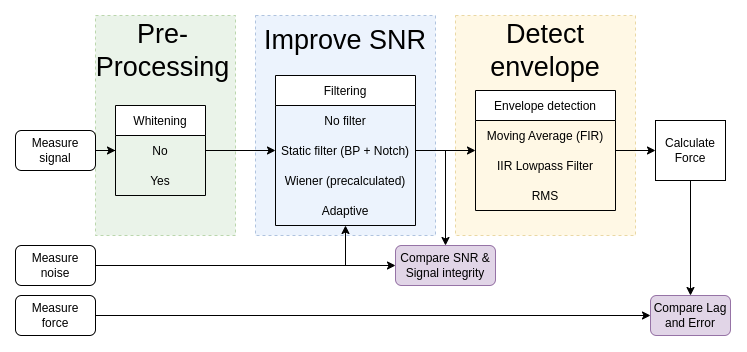
\includegraphics[height=60mm]{images/global_thesis_flowchart.png}
	\end{center}
	\caption{High-level overview of the signal processing chain}
	\label{fig:global_thesis_flowchart}
\end{figure}


\section{Approach}
The approach for this project consists of two main steps: Evaluate filter performance on sEMG signals, and evaluate the influence of whitening and different envelope extraction techniques on the lag and error of an estimated force signal.

The filters are assessed by signal to noise ratio (SNR) and signal integrity. Different envelope estimation techniques are evaluated by their lag and error compared to a simulated modulation. The combination of whitening, different filtering techniques, and different envelope extraction techniques is also evaluated through a measurement setup consisting of a 20kg load cell and a multi-channel EMG sensor. This setup is subsequently used to estimate the force from the sEMG signals and compare it to the force measured using the load cell.
\chapter{Theory}
The required background theory will be presented in a top-down approach. For someone experienced in the field of sEMG and signal processing some portions can be perceived as ubiquitous but it is done to make this paper more accessible for readers from different fields.

\section{Force estimation from sEMG}
When moving a limb the most intuitive way of describing it is a change in position, moving your hand from A to B. However, a more objective way of describing this movement is in terms of forces applied on a mass \cite{human_physiology,human_anatomy_physiology,3d_printing_soft_semg}:
\begin{itemize}
    \item The brain makes decision to move a limb and sends a signal through motor neurons
    \item The synaptic input received from the motor neuron results in contraction of the muscles
    \item This (simply put) causes a force to be applied on a mass, or a torque around a pivot point
    \item This force results in an acceleration in a certain direction
    \item This acceleration is maintained for a certain period of time
    \item The entire process is repeated for deceleration using visual, kinesthetic, proprioceptive and tactile sensory signals \cite{human_robotics}
    \item Your limb has arrived at a new location.
\end{itemize} 

Understanding this reasoning of moving a limb in terms of forces being applied by contracting muscles is vital because it forms the basis for recognizing a user's intent. EMG can be used to measure the intensity of muscle activation which indicates the amount of contraction \cite{human_robotics}. By measuring the amount of contraction of two antagonistic muscles it is possible to calculate the amount of force applied in a certain direction. Even if the limb is replaced by a prosthesis this idea of forces moving a mass will still apply, and thus EMG can be used as a human-machine interface.

So to summarize the basic concept of force estimation:
\begin{itemize}
    \item Movement of a limb is the result of a net force acting on that limb
    \item This net force is the result of certain muscles contracting stronger than other muscles
    \item The contraction of these muscles follows from muscle activation 
    \item Muscle activation can be measured using EMG
    \item EMG can be used to estimate limb movement
\end{itemize}

\begin{figure}[h!t]
	\begin{center}
		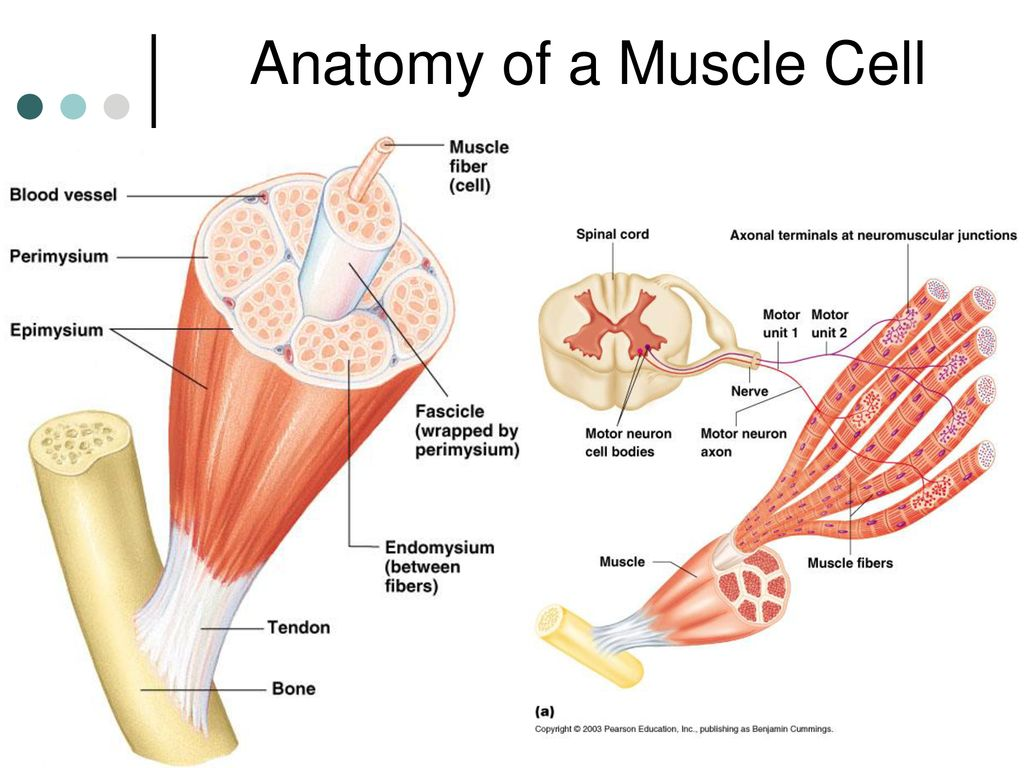
\includegraphics[width=0.7\columnwidth]{images/anatomy_of_a_muscle_cell.jpg}
	\end{center}
	\caption{Anatomy of a muscle \cite{human_anatomy_physiology}.}
	\label{fig:muscle_anatomy}
\end{figure}


Figure~\ref{fig:muscle_anatomy} illustrates the anatomy of a muscle. 
Large skeletal muscles such as the biceps consists of hundreds of thousands of small muscle fibers. These muscle fibers are divided into groups called motor units, and each motor unit is connected to a motor neuron which is a special type of very long brain cell that runs through the spinal cord. A contraction of a skeletal muscle is the result of many muscle fibers contracting individually and repeatedly \cite{human_anatomy_physiology}. The contraction of these muscle fibers is the result of muscle activation which in turn is the result of an action potential caused by the motor neuron. The activation of the muscle fibre is a small yet measurable voltage. When measuring the surface EMG of an activating skeletal muscle the result is the aggregate of the small voltages from all activating muscle fibers. This manifests itself into a signal resembling white noise where the amplitude of the noise correlates to the number of activated muscle fibers and thus to the amount of contraction the skeletal muscle will experiences \cite{optimal_myoprocessor}. An illustration of the form of the measured sEMG is shown in Figure~\ref{fig:sEMG_signal_example} where a maximum voluntary contraction (MVC) is measured from a biceps.
 
\section{sEMG signal properties}
\begin{figure}[h!t]
	\begin{center}
		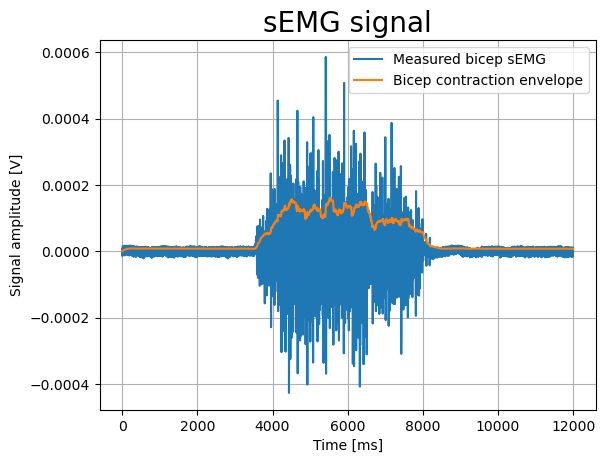
\includegraphics[width=0.7\columnwidth]{images/sEMG_signal_example.png}
	\end{center}
	\caption{sEMG signal measured from bicep during contraction}
	\label{fig:sEMG_signal_example}
\end{figure}

To summarize: to determine the degree of activation of a skeletal muscle we simply need to determine the amplitude of the noise at the surface of the muscle.

From this point onward 'noise' will refer to the generated by muscle contraction as 'the signal'. the reason for this is that noise is usually unwanted, but the signal caused by muscle contraction is the opposite of unwanted: It precisely what sEMG is trying to measure! 

Unfortunately, when measuring sEMG signals it is impossible to measure solely the signal generated by muscle contraction. The signal may be contaminated by other signals coming from the surrounding environment or from the amplifier used to amplify the measured signal. So in reality we are measuring a combination of our desired signal from muscle contraction, and the undesired noise from the environment and amplifier. An illustration of the frequency content of the signal and noise is shown in Figure~\ref{fig:sEMG_fft_signalnoise_example}. Note how the noise has large peaks at \SI{50}{\hertz} and multiples of \SI{50}{\hertz}; This is the noise generated by power lines nearby. 

\begin{figure}[h!t]
	\begin{center}
		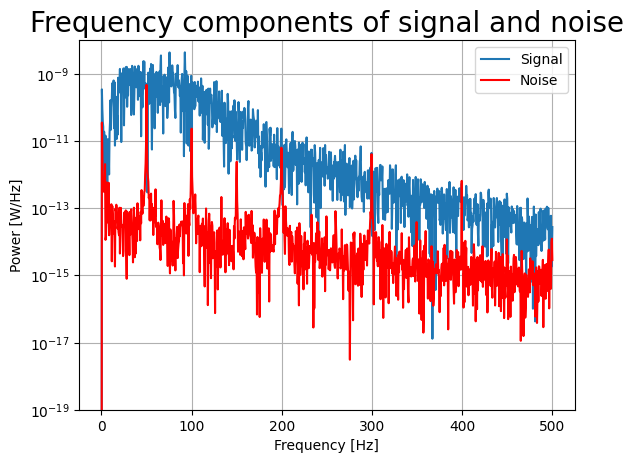
\includegraphics[width=0.7\columnwidth]{images/sEMG_fft_signalnoise_example.png}
	\end{center}
	\caption{Frequency components of signal and noise in an sEMG signal. 
    Noise is taken to be 0-2s and Signal is taken to be 5-7s in \ref{fig:sEMG_signal_example}}
	\label{fig:sEMG_fft_signalnoise_example}
\end{figure}

The ratio between how much of the measured signal is actual desired signal and how much is undesired noise is called the Signal to Noise Ratio (SNR) and is defined as the average signal power divided by the average noise power and can be seen in Equation~\ref{eq:snr} \cite{introduction_analog_digital_communications}. Intuitively one might think that force can be more accurately estimated from sEMG signals with a high SNR, this assumption will be tested in this report. SNR can be increased by removing noise from a noisy signal which can be done by a selection of tools called filters.

\begin{equation}\label{eq:snr}
    \text{SNR} = \frac{\text{Signal power}}{\text{Noise power}}
\end{equation}

\section{Filters}
% Introduce basic concept of filters
Filters are a tool that can be used to remove something unwanted (noise) that is mixed with something wanted (signal). In signal processing filtering is achieved by decomposing a measured signal into repeating patterns and subsequently deciding which patterns should be retained and which patterns should be removed. Figure~\ref{fig:filter_example} displays how a time-domain signal can be represented in the frequency domain to display information about which frequencies are present in the signal.

\begin{figure}[h!t]
	\begin{center}
		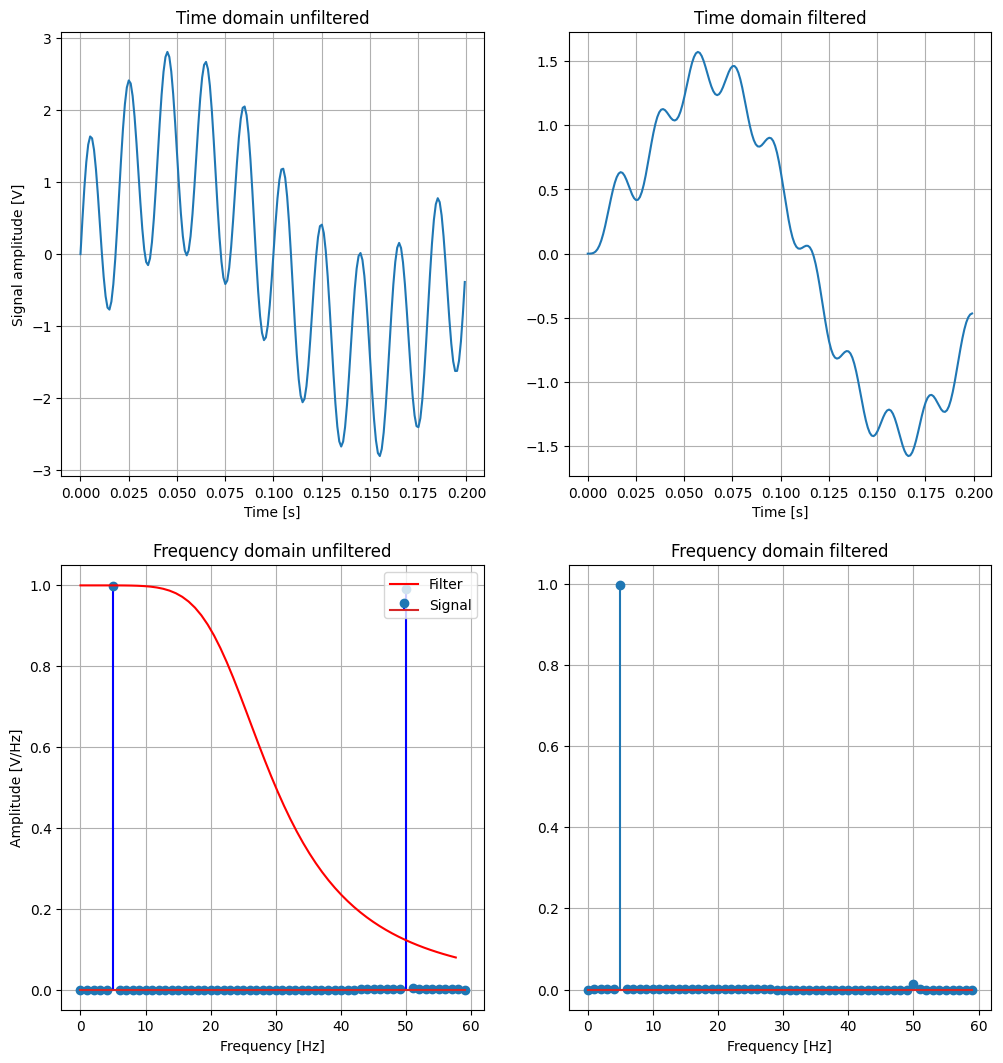
\includegraphics[width=1.0\columnwidth]{images/filter_example.png}
	\end{center}
	\caption{Filtering a signal. In the top-left figure there is a low-frequency signal polluted by a 50Hz signal. The frequency plot in the bottom-left shows these frequencies. By applying the low-pass filter as displayed in the bottom-left it is possible to filter out the higher \SI{50}{\hertz} frequency. The resulting filtered signal can be seen in the top-right, showing that there is still a little bit of noise left. This is also visible in the bottom right showing the frequency contents of the signal after filtering}
	\label{fig:filter_example}
\end{figure}

A digital filter consists of a set of values called the filter coefficients. The input (measurements) is multiplied with the filter coefficients to create the output. That is, the latest measurement is multiplied with the first filter coefficient, the previous measurement is multiplied with the second filter coefficient, and so on. This can also be interpreted as multiplying each filter coefficients with a delayed input sample. Figure~\ref{fig:wiki_digital_filter_working} shows the working and standard notation of a digital filter.
By carefully choosing the number and value of filter coefficients it is possible to attenuate specific frequencies while not influencing other frequencies such as the effect shown in \ref{fig:filter_example}. Analog signals and filters are conventionally presented as a continuous function of time (e.g. $x(t)$). Digital signals and filters are discrete rather than continuous, and are conventionally presented as a function of samples (e.g. $x(n)$). The variable $n$ describes the n'th sample of the signal. Converting a continuous signal to a discrete signal is done through the process of sampling the continuous signal at equidistant points in time: $s(n)=s(n*\Delta t)$ \cite{linear_systems_and_signals}.

\begin{figure}[h!t]
	\begin{center}
		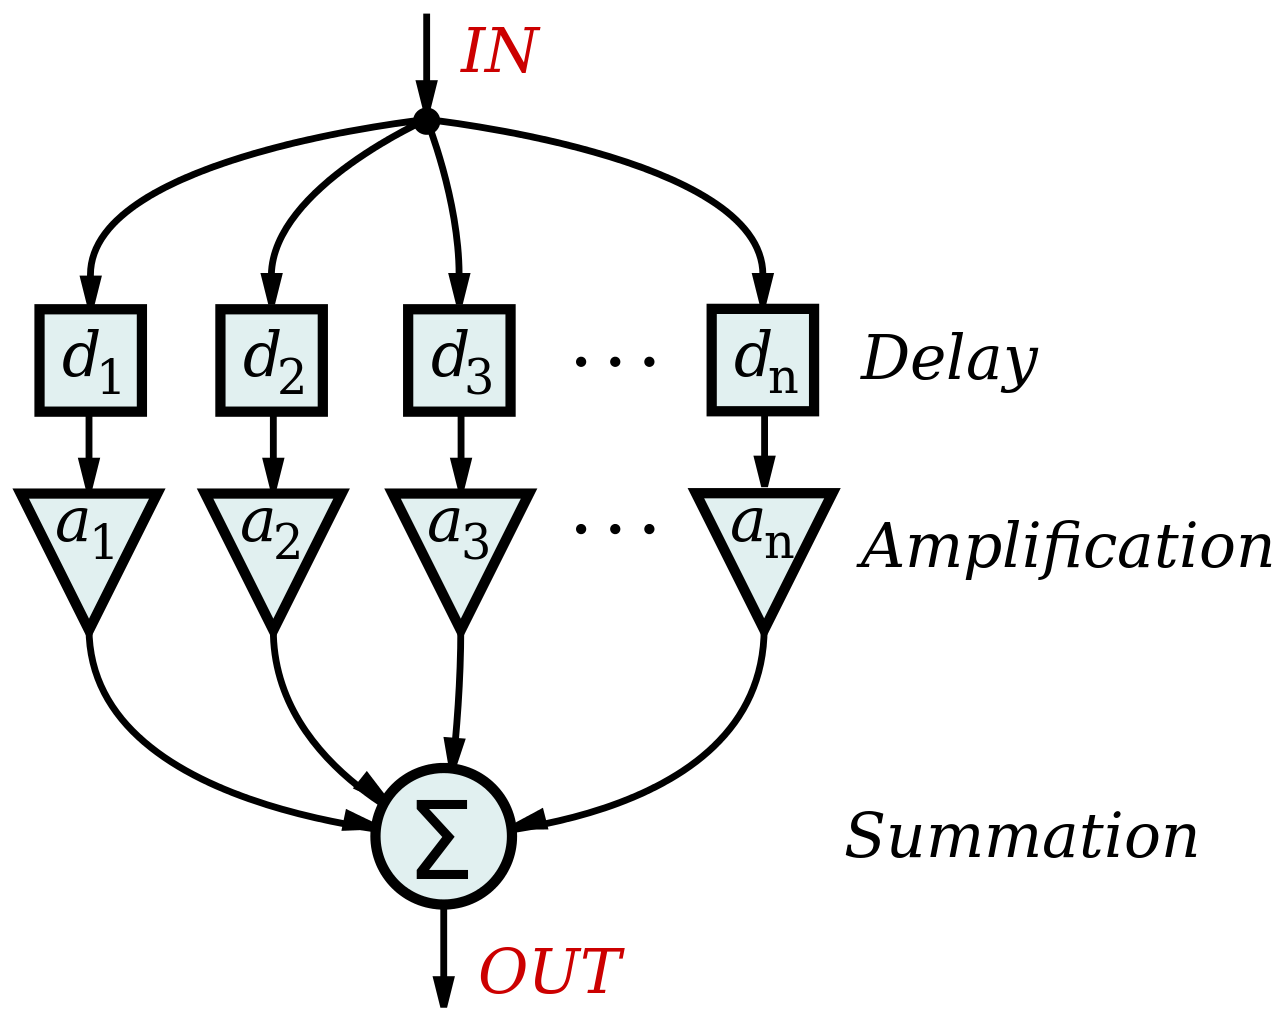
\includegraphics[width=0.4\columnwidth]{images/wikipedia_fir_digital_filter.png}
	\end{center}
	\caption{The functioning of a digital filter. The filter coefficient at index $i$ is multiplied by the input that is delayed $i$ samples \cite{wikipedia:digital_fir_filter_image}}
	\label{fig:wiki_digital_filter_working}
\end{figure}

\subsection{Static filters, Wiener filter, Adaptive filters}\label{sec:filters_theory}
The main difference between the different presented filter types is the way of calculating the filter coefficients. If a filter is static (e.g. high-pass, low-pass, band-pass, or band-stop) it simply means that the number of filter coefficients and the values of the filter coefficients are predetermined. These filters are very popular due to their simplicity in terms of finding the value of the filter coefficients. 

A Wiener filter aims to produce an estimate of a target process by linear time-invariant filtering of a noisy signal using knowledge of the spectrum of the stationary noise and target process assuming additive noise \cite{wiki:Wiener_filter,lecture_adaptive_filters_1}. Figure~\ref{fig:wiener_filter_diagram} shows the use of a Wiener filter. It is assumed that the noise component $v(n)$ is correlated to the noise component in the input signal in input $d(n)$ and uncorrelated to the desired signal $s(n)$. The Wiener filter coefficients aim to minimize the correlated signals, leaving only the desired signal as the 'error'. It is the optimal solution in terms of mean square error to statically filtering additive noise from a signal. The filter is constructed from the cross-correlation between an input sample and a noise sample, and the auto-correlation of the noise sample.

\begin{figure}[h!t]
	\begin{center}
		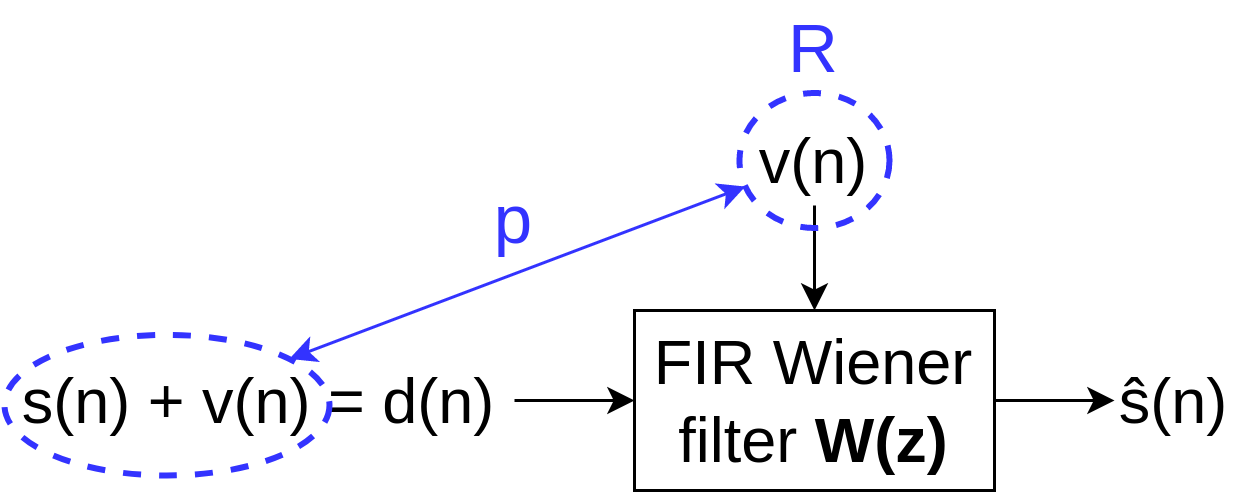
\includegraphics[width=0.7\columnwidth]{images/wiener_filter_diagram.png}
	\end{center}
	\caption{Diagram that illustrates the functioning of a Wiener filter. $s(n)$ is the desired signal, $v(n)$ is the additive noise, and $d(n)$ is the combination of desired signal and noise \cite{wiener_filter_system_identification}}
	\label{fig:wiener_filter_diagram}
\end{figure}

% $s(n)$ is the target signal, $v(n)$ is the additive noise. The goal of the Wiener filter is to find an estimate $\hat{s}(n)$ of the target signal $s(n)$ using spectral knowledge of $v(n)$ and of the additive combination of $s(n)+v(n)$. The target signal estimate $\hat{s}(n)$ is also called the 'error' as it is the part that is left over after applying the Wiener filter. $w$ presents the wiener filter coefficients.
%   \begin{equation}\label{eq:start_wiener}
%     \hat{s}(n) = (s(n) + v(n)) - \hat{v}(n) = d(n) - \boldsymbol{w}^T v(n)
%   \end{equation}
% Calculate the square of the error \cite{lecture_adaptive_filters_1}
% \begin{equation}
%     \hat{s}^2(n) = (d(n) - \boldsymbol{w}^T v(n))^2
% \end{equation}
% Expanding the brackets
% \begin{equation}
%     \hat{s}^2(n) = d^2(n) - 2d(n)\boldsymbol{w}^T v(n) + \boldsymbol{w}^T v(n)\boldsymbol{w}^T v(n)
% \end{equation}
% \begin{equation}
%     \hat{s}^2(n) = d^2(n) - 2 \boldsymbol{w}^T d(n) v(n) + \boldsymbol{w}^T v(n) v^T(n) \boldsymbol{w}
% \end{equation}
% Take the mean of both sides to end up with the Mean Square Error (MSE) \cite{lecture_adaptive_filters_1}
% \begin{equation}\label{eq:wiener_final}
%     E\left(\hat{s}^2(n)\right) = E\left(d^2(n)\right) - 2 \boldsymbol{w}^T E\left(d(n) v(n)\right) + \boldsymbol{w}^T E\left(v(n) v^T(n)\right) \boldsymbol{w}
% \end{equation}

% Redefine the terms of Equation~\ref{eq:wiener_final} to give insight into their definitions \cite{lecture_adaptive_filters_1}
% \begin{align}
% &J(\boldsymbol{w}) \                  &=& E(\hat{s}^2(n))  &=& \text{MSE (scalar)} \label{eq:wiener_mse_def}\\
% &\sigma^2 \           &=& E(d^2(n))        &=& \text{Power of }d(n) \text{ (scalar)} \\
% &\boldsymbol{p} \      &=& E(d(n) v(n))     &=& \text{M-by-1 Cross-correlation vector between } d(n) \text{ and } v(n)  \\
% &\boldsymbol{R} \      &=& E(v(n) v^T(n))  &=& \text{M-by-M Auto-correlation matrix of } v(n)
% \end{align}

% Substitute these terms into Equation~\ref{eq:wiener_final} to form the total equation for Mean Square Error \cite{lecture_adaptive_filters_1}
% \begin{equation}
%     J(\boldsymbol{w}) = \sigma^2 - 2 \boldsymbol{w}^T \boldsymbol{p} + \boldsymbol{w}^T \boldsymbol{R} \boldsymbol{w}
% \end{equation}
% To find the filter coefficients that result in minimum MSE we take the derivative of the MSE with respect to each filter coefficient. The derivation of this process is quite lengthy but can be found in \cite{proakis_manolakis_1996}. The resulting final solution is called the Wiener-Hopf equation \cite{lecture_adaptive_filters_1} and is also shown in Equation~\ref{eq:wiener_hopf}
% \begin{equation}\label{eq:end_wiener}
%     \frac{\delta J}{\delta w_i} = 0, i = 0, 1, ... M-1 \ \rightarrow \ \boldsymbol{R} \boldsymbol{w_\text{opt}} = \boldsymbol{p} \ \rightarrow \ \boldsymbol{w_\text{opt}} = \boldsymbol{R}^{-1}\boldsymbol{p} \text{\cite{lecture_adaptive_filters_1}}
% \end{equation}


% The mathematical derivation for finding the optimal filter coefficients is given in equations \ref{eq:start_wiener} to \ref{eq:end_wiener}. The conclusion is that the optimal filter coefficients are calculated by multiplying (dot-product) the inverse of the auto-correlation of signal+noise and the cross-correlation between signal+noise and noise. 
In sEMG, the signal+noise is measured at the point of muscle contraction while the noise can be measured separately from a different body part that does not experience contraction. This separately measured noise has similar frequency characteristics as the noise included in the signal+noise as it experiences the same amplifier noise and environment noise. The resulting frequency domain definition of the optimal Wiener filter is defined in Equation~\ref{eq:wiener_filter_frequency_behaviour}\cite{stanford_wiener_filter}. $\Phi_\text{s}(z)$ reflects the frequency contents of signal+noise, and $\Phi_\text{v}(z)$ reflects the frequency contents of the noise.

\begin{equation}
    H_\text{opt}(z) = \frac{\Phi_\text{s}(z)}{\Phi_\text{s}(z) + \Phi_\text{v}(z)}
    \label{eq:wiener_filter_frequency_behaviour}
\end{equation}

Assuming that the calculated Wiener filter approximates the optimal Wiener filter, multiplying the filter (in frequency domain) with the signal+noise input will result in an approximation of the signal as seen below.

\begin{align}
    \hat{\Phi_\text{s}}(z) & \ = \ \hat{H_\text{opt}}(z) \ \cdot \ (\Phi_\text{s}(z) + \Phi_\text{v}(z)) \label{eq:wiener_filter_frequency_application_1} \\
    & \ = \ \frac{\hat{\Phi_\text{s}}(z)}{\hat{\Phi_\text{s}}(z) + \hat{\Phi_\text{v}}(z)} \ \cdot \ (\Phi_\text{s}(z) + \Phi_\text{v}(z)) \label{eq:wiener_filter_frequency_application_2}\\
    & \ \approx \ \Phi_\text{s}(z) \label{eq:wiener_filter_frequency_application_3}
\end{align}

The Wiener filter requires both the signal and the noise to be stationary, i.e. the spectral density does not change over time, and results in a linear time-invariant filter \cite{stationary_processes_definition} \cite{difference_stationary_nonstationary}. If the signal and noise were not stationary then the approximated frequency spectrum of signal+noise is not the same as the actual frequency spectrum of signal+noise which means they no longer cancel out in Equation~\ref{eq:wiener_filter_frequency_application_2} and Equation~\ref{eq:wiener_filter_frequency_application_3} no longer holds.
As an example a Wiener filter was made from the signal as seen in Figure~\ref{fig:sEMG_signal_example}. The time span from \SIrange{0}{2}{\second} is taken as the 'noise', and the time span from \SIrange{5}{7}{\second} is taken to be signal+noise. From these a Wiener filter is constructed and can be seen in Figure~\ref{fig:wiener_filter_response}.

\begin{figure}[h!t]
	\begin{center}
		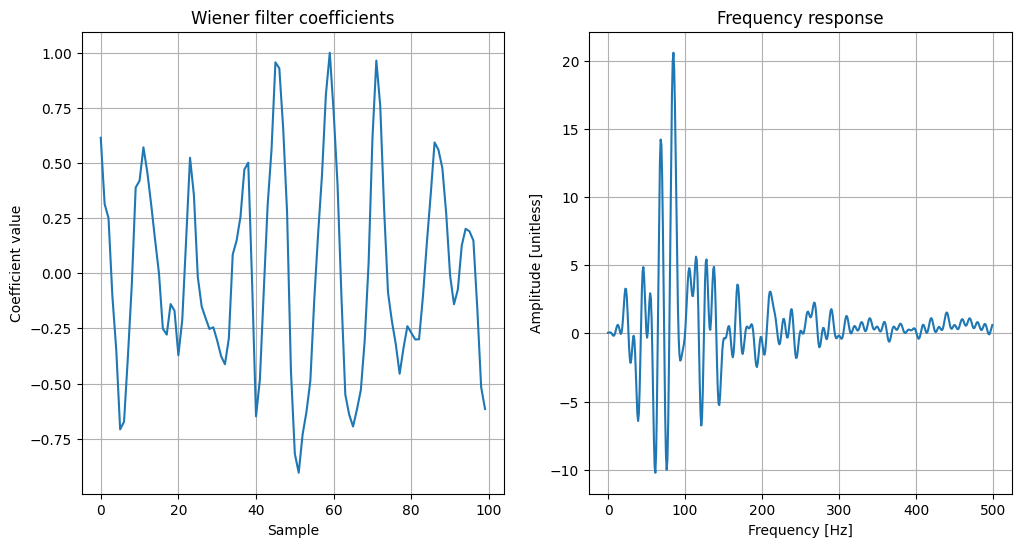
\includegraphics[width=1.0\columnwidth]{images/wiener_filter_response.png}
	\end{center}
	\caption{Sample values and frequency responses of a Wiener filter}
	\label{fig:wiener_filter_response}
\end{figure}

\begin{figure}[h!t]
	\begin{center}
		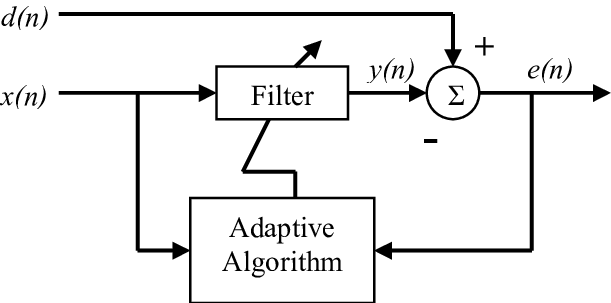
\includegraphics[width=1.0\columnwidth]{images/adaptive_filter_block_diagram.png}
	\end{center}
	\caption{Block diagram of an adaptive filter \cite{introduction_optimal_signal_processing}}
	\label{fig:adaptive_filter_diagram}
\end{figure}

Adaptive filters is a class of filters where the filter coefficients are adjusted over time to attempt to find an optimal solution even without knowing the spectral properties of the signal beforehand \cite{adaptive_filter_and_applications}. Adaptive filters adjust the filter coefficients by decreasing the error that remains after applying the filter. A diagram describing this process can be found in Figure~\ref{fig:adaptive_filter_diagram}. 
One type of adaptive filter is the Least Mean Square (LMS) algorithm. Where a Wiener filter finds an optimal solution by using cross-correlation and auto-correlation, the adaptive LMS algorithm converges to the optimal solution (i.e. the solution found by the Wiener filter given complete knowledge of the spectral domain) using gradient descent. Filter coefficients will never reach $w_\text{opt}$ but instead oscillate around it. The mathematical definition for calculating the filter coefficients is given, derived from the work of J. Orfanidis \cite[Ch. 7.3]{introduction_optimal_signal_processing} and lectures by S. Safapourhajari \cite{lecture_adaptive_filters_2}. Again it is assumed that there is an input signal ($d(n)$) consisting of a desired signal ($e(n)$) and additive noise ($x(n)$), as well as a separate measure of the noise that is correlated with the noise in the input signal but uncorrelated with the desired signal.

The cost function for adjusting the adaptive filter as seen in figure \ref{fig:adaptive_filter_diagram} coefficients is taken to be the Mean Square Error $J$ (MSE):
\begin{equation}
    J(w) = E(e^2(n)) = E[(d(n) - wx(n))^2)]
\end{equation}
To calculate the expected value of the square of the error we would normally need statistics over a large block of data. An approximation of the expected value can be made by using a smaller set of data. This can be done by taking the current samples as the estimates of the mean
\begin{equation}
    E(e^2(n)) \sim e^2(n)
\end{equation}
Since the error $e(n)$ equals $d(n) - wx(n)$ this can be filled into the equation
\begin{equation}
    E((d(n) - wx(n))^2)) \sim (d(n) - wx(n))^2
\end{equation}

To find $w$ that minimizes the MSE we can take the derivative of MSE with respect to $w$ for every sample $n$
\begin{equation}
    \frac{\delta J}{\delta w} = 2(d(n) - wx(n)) \frac{\delta(d(n) - wx(n))}{\delta w} = -2e(n)x(n)
\end{equation}
This results in the following weight-adjusting algorithm
\begin{align}
    \textrm{w(n+1)}&=\left.w(n)-\mu \frac{\delta J}{\delta w}\right\rvert_\text{\textrm{w(n)}} \\
    &= w(n) + 2 \mu e(n)x(n)
\end{align}


This algorithm is implemented by performing the following steps. \\
The estimated value for signal+noise is computed from the filter and noise
\begin{equation}\label{eq:adaptive1}
    \hat{x}_n = w(n)\cdot y(n)
\end{equation}
The error is calculated by taking the difference between the expected signal+noise value and the measured signal+noise value.
\begin{equation}\label{eq:adaptive2}
    e(n) = x(n) - \hat{x}_n
\end{equation}
The coefficients are calculated for the next iteration
\begin{equation}\label{eq:adaptive3}
    w(n+1) = w(n) + 2 \mu e(n) x(n)
\end{equation}

The steps in equations \ref{eq:adaptive1}-\ref{eq:adaptive3} are repeated for every sample.

In the presented equations a constant $\mu$ was present, this is called the convergence coefficient. Determining the value of the convergence coefficient $\mu$ is a double-edged sword. On the one hand it determines how fast gradient descent is traversed, and thus how fast the filter coefficients converge to the optimal filter coefficients. Ideally this happens as fast as possible, and thus the convergence coefficient must be as large as possible. On the other hand it was previously mentioned that the filter coefficients will never reach the optimal filter coefficients but instead oscillate around this value. The convergence coefficient also determines how large this oscillatory behaviour is, and thus to achieve an accurate estimation of the optimal filter the convergence factor should be as small as possible. 

A problem presented by the basic LMS algorithm is that scaling the input also results in scaling the error term calculated in Equation~\ref{eq:adaptive2}. This makes it difficult (if not impossible) to find a convergence factor that functions across a wide range of possible scaled inputs. A solution to this problem is found in the work of Haykin \cite{adaptive_filter_theory} in the form of the Normalized LMS filter. This normalizes the power of the input signal before multiplying the input with the error and convergence factor. This is done by dividing the input signal with the the dot product of the input signal with itself. It turns Equation~\ref{eq:adaptive3} into Equation~\ref{eq:adaptive4} \cite{adaptive_filter_theory}.

\begin{equation}\label{eq:adaptive4}
    w(n+1) = w(n) + 2 \mu e(n)  \frac{x(n)}{x(n) \cdot x(n)}
\end{equation}

Common applications of adaptive filters include speech recognition, echo cancellation, and headphones employing active noise cancellation \cite{active_noise_cancellation_wiener_filter,wiener_vs_adaptive_realtime_noisecancellation}.

\subsection{FIR vs IIR}
Another subdivision within filter design is concerned with the type of possible responses to a specific input (impulse) and whether or not this can go to infinity.

The previously discussed filters were all described as Finite Impulse Response (FIR) filters. This means that the output is the result of multiplying the filter coefficients with the input. This type of filter is always stable and the output can never go to infinity as long as the input does not go to infinity.

An Infinite Impulse Response filter calculates the output using two sets of filter coefficients. The first set of filter coefficients is used to multiply with the input just like a FIR filter, but the second set of filter coefficients is used to multiply with previous \textit{outputs}. This means that there is now a feedback loop in the system, and a system with feedback can become unstable. Unstable in this case means that there is a possibility of positive feedback loop where increasing output values result in future output values also increasing, eventually going to infinity. Even though this feedback and possible instability may sound like a downside, it also results in shorter filter length and thus fewer computations required per filter operation. This could especially provide beneficial in low memory and low compute power environments like in prostheses \cite{fir_vs_iir}.

Both static and adaptive filters can be implemented as both FIR or IIR filters. An adaptive IIR filter offers the potential to meet desired performance levels with much less computational complexity. However, the possibility for the system to become unstable combined with the fact that filter coefficients are adjusted automatically leads to a high-risk high-reward scenario due to a loss of control and hard to predict behaviour \cite{digital_signal_processing_handbook}.

\begin{figure}[h!t]
	\begin{center}
		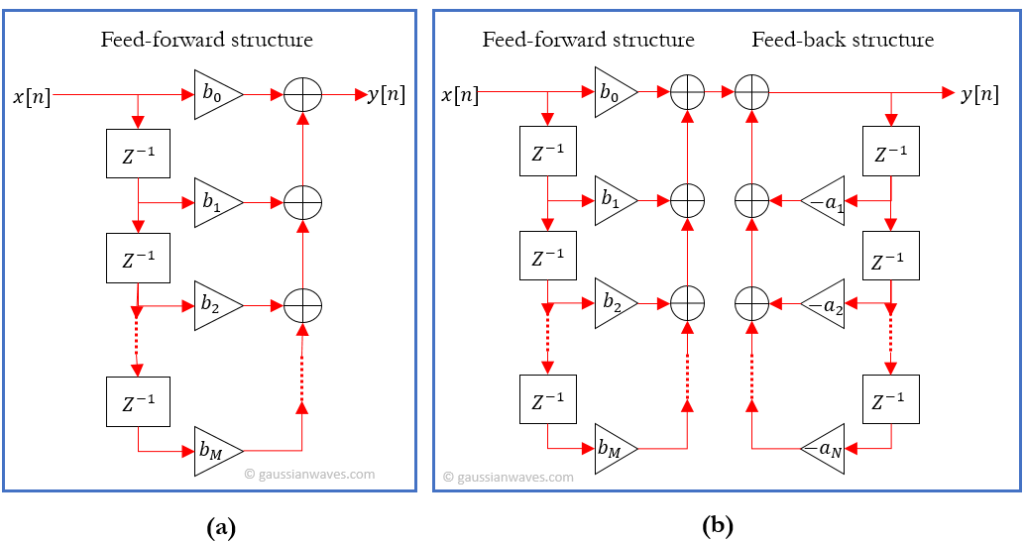
\includegraphics[width=1.0\columnwidth]{images/fir_vs_iir_diagram.png}
	\end{center}
	\caption{A diagram displaying the difference between Finite impulse response filters, only using previous input, and Infinite impulse response filters, using previous inputs and previous outputs resulting in a feedback loop \cite{fir_vs_iir_diagram}}
	\label{fig:fir_vs_iir_diagram}
\end{figure}


\section{Pre-whitening}
During literature research it was noticed that it was not uncommon for literature to mention something along the lines of "including a temporal whitening filter [...] improves the performance of the amplitude estimate" \cite{single_site_emg_amplitude_estimation,adaptive_whitening,emg_whitening}. However, an intuitive explanation of \textit{why} whitening works was consistently lacking. So to understand the reasoning behind whitening we need to take a short detour to the world of computer science and information theory.

Back in 1948 a mathematician, electrical engineer, and cryptographer named C.E. Shannon published a pioneering paper that formed the basis of information theory \cite{shannon}. In this paper it is shown that repetition does not carry information, and that the maximum information transfer occurs when a signal is truly random. Imagine a signal with only a single frequency component. After measuring a few samples of the signal the conclusion is drawn that this is a \SI{50}{\hertz} signal. Since it is possible to predict the value of every future measurement of the signal after drawing this conclusion it becomes unnecessary to continue measuring the signal because it will not give any new information. A repeating pattern is predictable, and predictable events carry no information.

The polar opposite of a signal containing a single frequency (and therefore predictable and carries little information) is a signal that contains all frequencies an equal amount. This is called a white noise signal and carries the maximum amount of information because there exists no repetition and therefore every sample carries new, unpredictable information.

Between the existence of a signal containing a single frequency, and a signal containing all frequencies (white noise), all other signals exist and have certain frequencies that are more 'present' than other frequencies. These signals have different degrees of predictability (and thus information density), and the degree of predictability is determined by how closely the frequency content resembles white noise.

Whitening is a filtering technique that tries to equalize the presence of frequency components in a signal to approximate white noise and thus increase information density. It reduces the random error and yields a larger dynamic range because the small frequency components that contribute to the 'randomness' of the signal but not so much to the value of the measurement sample become more present \cite[Ch. 5.4.9]{time_series_analysis_methods}\cite{single_site_emg_amplitude_estimation}. The serial correlation of the signal is decreased by reducing the presence of 'predictable' signals, which increases the randomness and thus information density \cite{serial_correlation_definition}. 

This previous information manifests itself in sEMG signal processing by the fact that the measured sEMG signal is not white. Some frequency components are much more present than others, but all frequencies equally contribute to the indication of muscle contraction. To get a more accurate indication of muscle contraction the signal should be whitened to increase the information of each sample.

Whitening in real-time is achieved through a digital filter with a frequency response that when multiplied with the sEMG signal frequency spectrum yields a white noise spectrum.

To summarize: Whitening reduces the power of repeating frequencies and increase the power of random frequencies in the signal. An example is given in Figure~\ref{fig:whitening_example}.

\begin{figure}[h!t]
	\begin{center}
		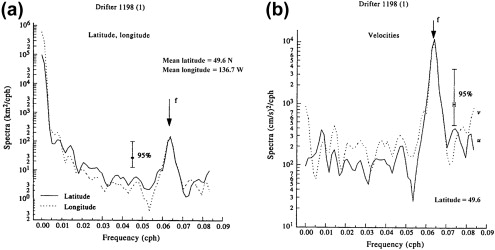
\includegraphics[width=1.0\columnwidth]{images/prewhitening_example.jpg}
	\end{center}
	\caption{An example of whitening a signal. The indicated peak contains the 'random' signal of interest. By whitening the powerful lower frequencies it is possible to give the information-carrying peak more presence on the signal \cite{time_series_analysis_methods}}
	\label{fig:whitening_example}
\end{figure}


\section{Envelope detection}

\begin{figure}[h!t]
	\begin{center}
		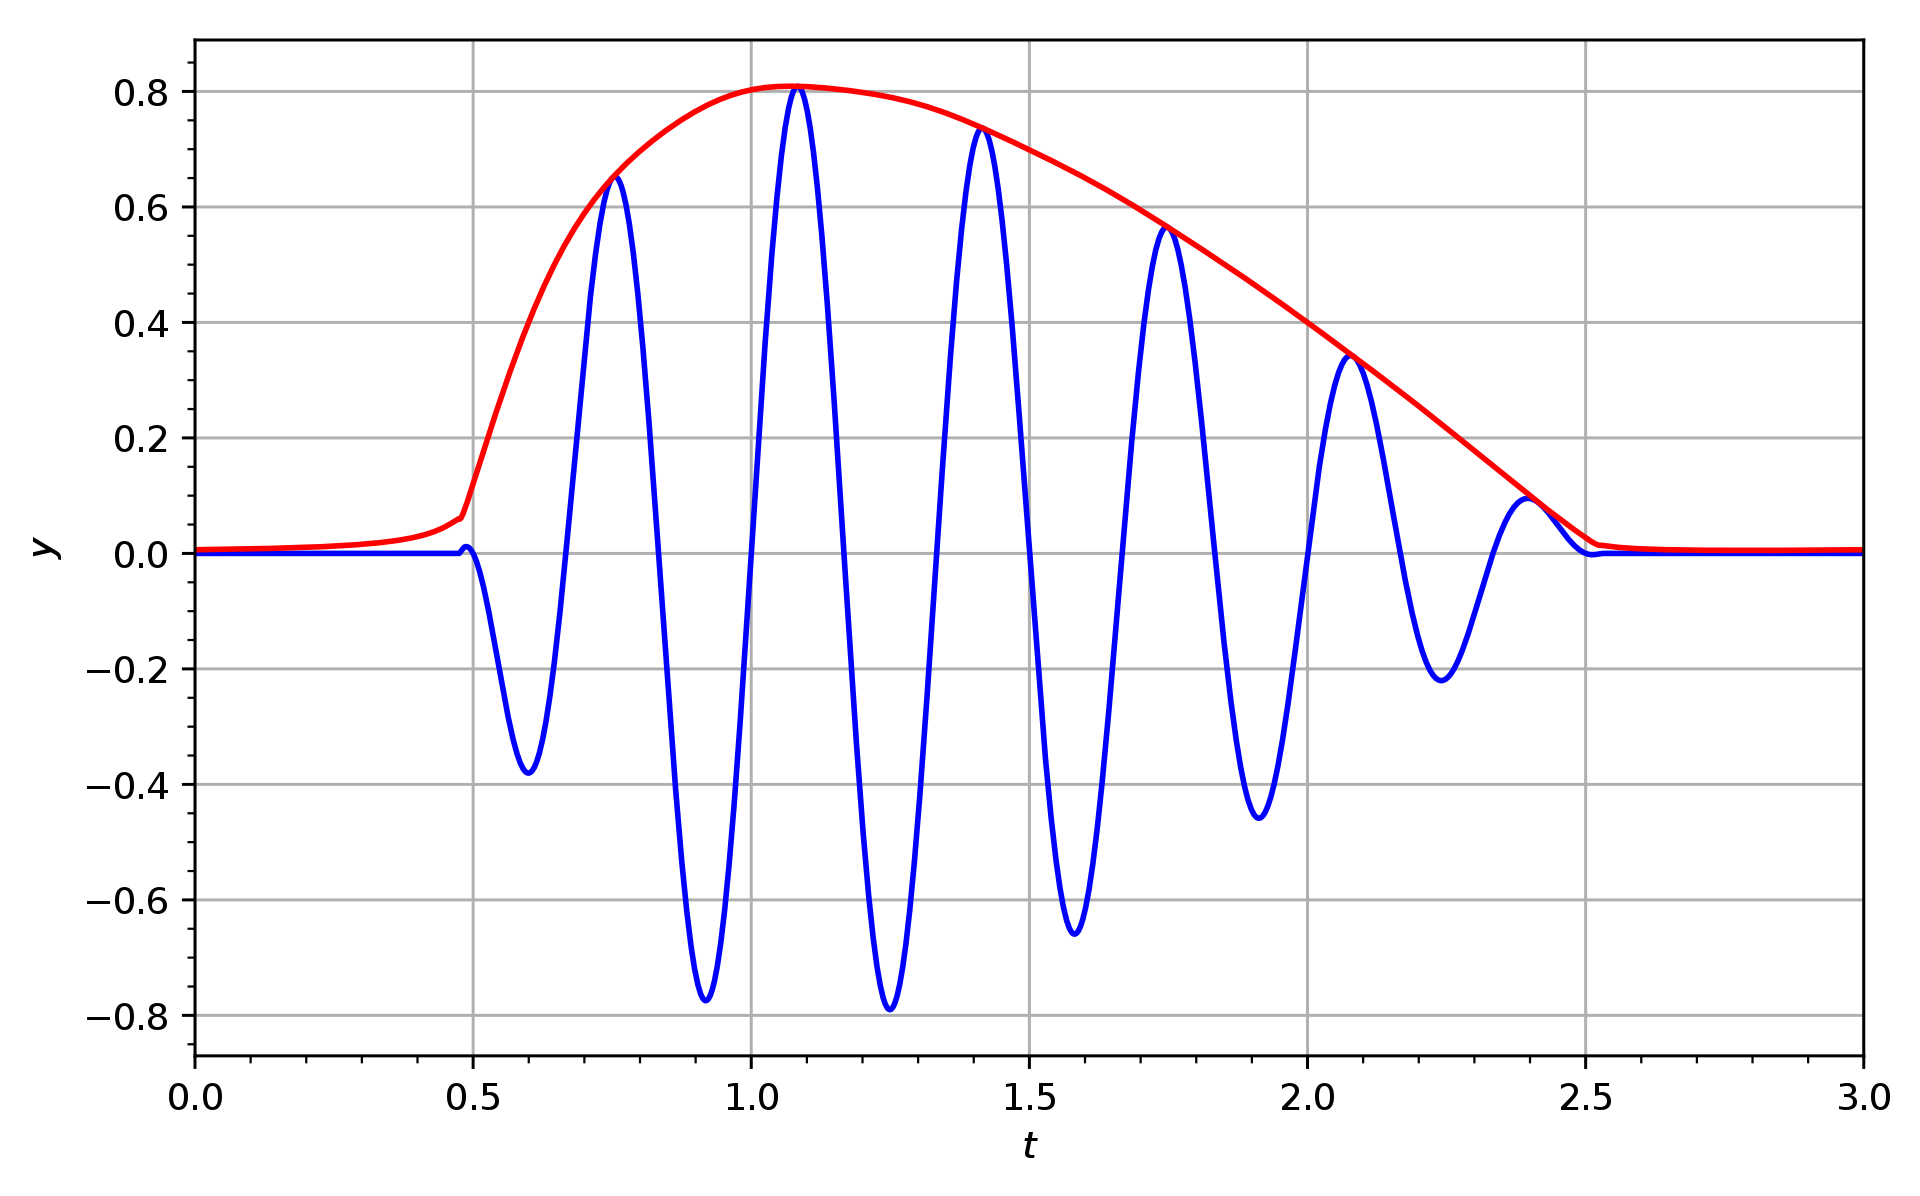
\includegraphics[width=0.7\columnwidth]{images/envelope_wikipedia.png}
	\end{center}
	\caption{Illustrating envelope detection of an analytical signal \cite{envelope_wikipedia}}
	\label{fig:envelope_wikipedia}
\end{figure}

\begin{figure}[h!t]
	\begin{center}
		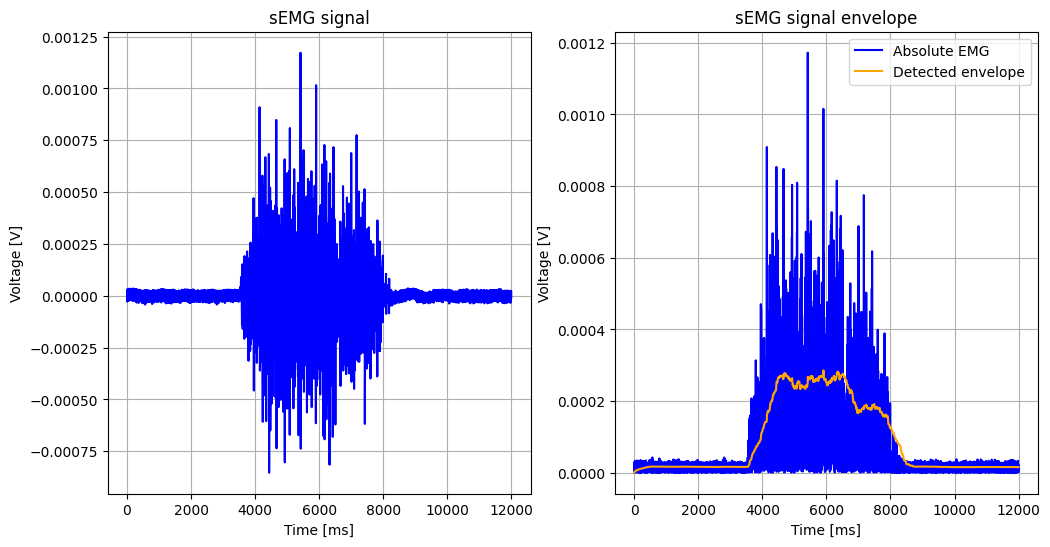
\includegraphics[width=1.0\columnwidth]{images/amplitude_force_estimation_example.png}
	\end{center}
	\caption{On the left a time-domain sEMG signal. On the right an example of envelope estimation is presented. By taking the absolute value of the sEMG signal on the left and calculating the envelope it is possible to make an estimation of muscle contraction. The next step would be force estimation but this requires two antagonistic muscles. This is discussed more in-depth in section \ref{section:force_estimation}}
	\label{fig:amplitude_estimation_example}
\end{figure}

The relation between the amplitude of a measured sEMG signal, the degree of contraction of a skeletal muscle and the exerted force is very complicated. However, the relationship between force and EMG amplitude during isometric contractions is usually linear or close to linear  \cite{interpreting_muscle_function_from_emg} \cite{adaptive_filter_dry_electrode}. This is the reason that in this report it is assumed that there exists a linear relation between force and sEMG signals.

Since the raw EMG signal consists of stochastic and unpredictable noise it is difficult to draw conclusions about the degree of muscle contraction when solely looking at individual samples \cite{semg_signals_analysis_and_applications}. By drawing an outline of the peaks of the signal a much more informative picture can be drawn. This is called an envelope and an illustration of this process can be found in Figure~\ref{fig:envelope_wikipedia}. In the case of more random sEMG signals it is preferred to perform full wave rectification on the signal before calculating the envelope so that all of the signal energy is taken into account \cite{semg_signals_analysis_and_applications}. Applying this concept to an sEMG signal can be found in Figure~\ref{fig:amplitude_estimation_example}.

Computationally envelope detection can be achieved in a number of different methods where "speed", or how much the detected envelope lags behind the true signal envelope, is traded against accuracy or noisiness \cite{dsp_good_bad_ugly}. A few different envelope detection techniques are discussed in \cite{rose2011electromyogram}.

\subsection{Moving average}
A moving average filter is a special type of FIR filter with coefficients that all have the value of $\frac{1}{n}$ where $n$ is the number of samples over which the average is taken. Thus the value of every smoothed sample is calculated to be the average of the previous $n$ samples. The upside of a moving average filter is that it introduces no phase distortion \cite{fir_filter_properties}, is very simple to implement, and require only addition to apply which is much faster than multiplication \cite{smith_moving_average_filters}. An illustration of the phase shift of a moving average filter is shown in Figure~\ref{fig:movingaverage_phaseshift}. An intuitive downside of a moving average filter is that its output lags behind the signal: a change in a static signal level is only properly reflected after $n$ samples. The sEMG signal must also be rectified before this method can be applied because EMG signal has approximately zero mean due to its oscillatory behaviour \cite{rose2011electromyogram}.

\begin{figure}[h!t]
	\begin{center}
		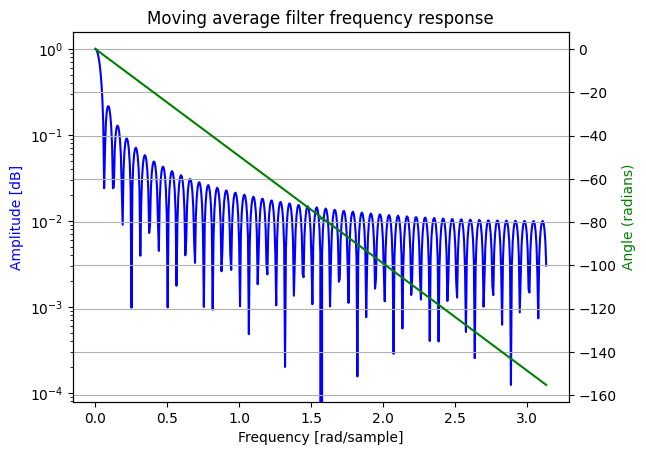
\includegraphics[width=0.7\columnwidth]{images/movingaverage_phaseshift.png}
	\end{center}
	\caption{Frequency response of a moving average filter. This particular filter consists of 100 coefficients all equal to 0.01. Notice how the filter has linear phase which indicates that there is no phase distortion due to the time delay of frequencies relative to another \cite{fir_filter_properties}}
	\label{fig:movingaverage_phaseshift}
\end{figure}



\subsection{IIR Low-pass filter}
A low-pass filter such as a Butterworth or Chebyshev can be used to determine the envelope of a rectified signal in a more 'responsive' (less lag) method compared to a moving average filter. The downside of this filter is that it introduces phase shift (as can be seen in Figure~\ref{fig:iirfilter_phaseshift}) unless applied in forward and backward direction \cite{rose2011electromyogram} which is not possible in real-time signals without introducing a static delay of a number of samples that equals the number of filter coefficients.

\begin{figure}[h!t]
	\begin{center}
		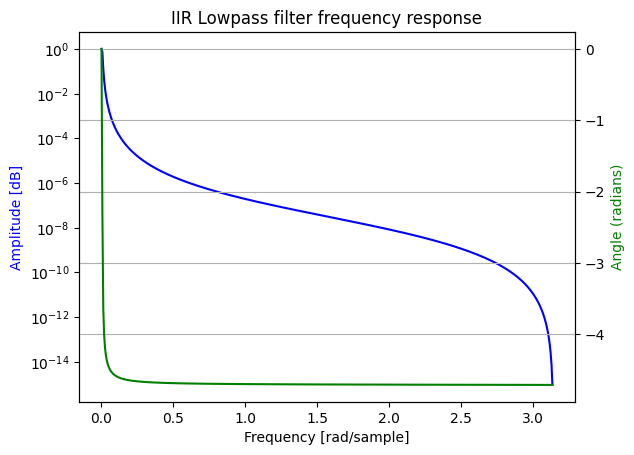
\includegraphics[width=0.7\columnwidth]{images/iirfilter_phaseshift.png}
	\end{center}
	\caption{Frequency response of an infinite impulse response (Butterworth) low-pass filter. The filter has a $f_\text{cut}$ of \SI{1}{Hz} and has a length of 3. Notice how the phase delay is \textit{not} linear and thus phase distortion is introduced}
	\label{fig:iirfilter_phaseshift}
\end{figure}

\subsection{Root Mean Square}
The Root Mean Square (RMS) of a signal is the square root of average power of a signal for a given period of time, a definition is given in Equation~\ref{eq:rms}. A useful property of RMS is that when it is applied to a signal with Gaussian distribution the RMS amplitude of the source is the same as the standard deviation of the distribution \cite{rms_standard_deviation}. In other words this means that RMS can extract the signal power of all frequencies in a signal in the time-domain if the frequencies are normally distributed. Since the probability density of surface EMG is approximately Gaussian, RMS should theoretically be the maximum likelihood estimator of EMG amplitude \cite{semg_signals_analysis_and_applications}.

\begin{equation}
    RMS = \sqrt{\frac{1}{n} (x[1]^2 + x[2]^2 + \cdots + x[n]^2)}
    \label{eq:rms}
\end{equation}

\section{Standard sEMG signal processing}\label{section:standard_semg_processing}
A conventional static real-time sEMG signal processing chain is described in \cite{muscle_force_estimation}. The relevant steps are as follows:
\begin{itemize}
    \item Remove DC component from signal
    \item Band-pass filter 20-\SI{300}{\hertz}
    \item Notch filter at \SI{50}{\hertz}
    \item Half-wave rectification
    \item Low-pass filter for envelope detection
\end{itemize}

This signal processing chain will also be tested in this report and compared to alternative techniques.

\section{Conclusion}
In this theory section the required background information is given to understand the simulations, measurements, and conclusions that will be drawn in this report. For each processing step, multiple processing methods have been discussed all of which can be seen in Figure~\ref{fig:global_thesis_flowchart}, and information about the relevant parameters has been given. For the Wiener filter and the adaptive LMS filter a mathematical derivation is presented.
\chapter{Simulation}
This section of the report describes the testing of separate signal processing steps in a simulated environment. Each block as seen in Figure~\ref{fig:global_thesis_flowchart} will be tested individually, and the method and results will be discussion on a per-block basis:
\begin{itemize}
    \item Pre-whitening
    \item Filtering
    \item Envelope estimation
\end{itemize}

Unless specified otherwise all signals will be high-passed with an $f_{cut}$ of \SI{1}{\hertz} to remove DC bias before any operation is applied

\section{Pre-whitening}\label{sec:whitening}
A whitening filter is a digital filter with a frequency response that is (ideally) the inverse of the frequency contents of an sEMG signal. 

\subsection{Method}
A testing signal was created that approximates the frequency response of an sEMG signal. The testing signal was created by creating a long white noise signal and multiplying the amplitudes in the frequency spectrum with a curve that estimates the frequency response of an sEMG signal. After this the signal is passed through inverse fft to go back to a time-domain signal. The result can be seen in \ref{fig:whitening_simulation} subplot 1 and 2.

The whitening filter is then created by taking the FFT of the time-domain test signal and taking its reciprocal at every frequency. Lastly the whitening filter frequencies are multiplied by the mean of the original signal frequencies to make sure that when the filter is applied the mean stays the same. These steps can be seen in \ref{fig:whitening_simulation} subplot 3. 

\subsection{Results}
\begin{figure}[h!t]
	\begin{center}
		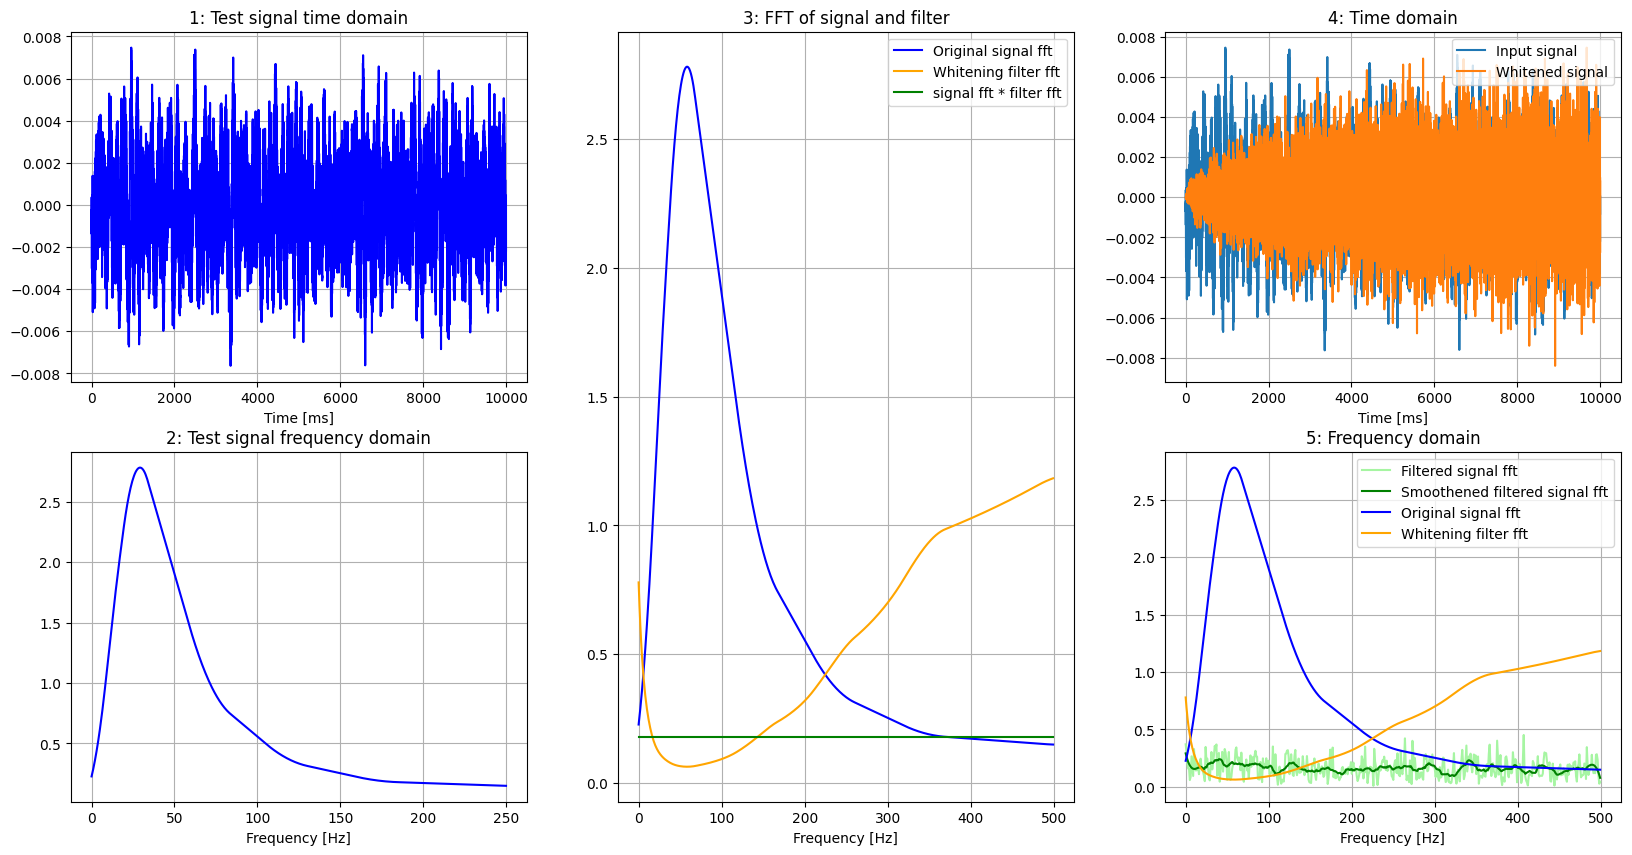
\includegraphics[width=1.0\columnwidth]{images/prewhitening_simulation.png}
	\end{center}
	\caption{Subplot 1 and 2 display the input simulated input signal with a frequency response that approximates the frequency contents of an sEMG signal. Subplot 3 displays the frequency content of the signal, the subsequently calculated whitening filter, and the multiplication of the signal with the filter in frequency domain to show that the response is indeed white. Subplot 4 and 5 show the original and 'whitened' signal in time domain and frequency domain.}
	\label{fig:whitening_simulation}
\end{figure}

Figure~\ref{fig:whitening_simulation} shows the whitening filter that functions as expected. In the center subplot the 'ideal' result are shown (multiplication in the frequency domain), and in subplot 5 the result from convolution in the time domain is shown. In subplot 5 a smoothed version of the filtered signal FFT is added to display that the signal power has a mean that approximates white noise. This filter was made using a Savitzky-Golay filter with a window length of 31 and a polynomial order of 3.

\section{Filtering}
First the metrics are introduced that will be used to compare filter performance. Subsequently, the construction process of each filter is presented. Lastly the different filtering methods are compared.

\subsection{Comparison metrics}
Each filter will be tested using two metrics: SNR (eq \ref{eq:rms}) and Bandwidth (definition of this will be given shortly). All filters are linear time invariant which means the superposition principle can be used to simplify SNR calculations \cite{linear_systems_theory}. The superposition principle simply states that filtering the sum of two signals is the same as filtering the signals individually and adding the results. An illustration of this can be seen in \ref{fig:filter_process}. 

Due to the difficulty of creating a simulated signal that has the frequency contents of an sEMG signal and environmental noise, a pre-recorded sample of sEMG of a bicep going through maximum voluntary contraction was used to test the filters. This sample is not used for force estimation because there is no way to validate the degree of contraction, and purely the frequency contents of the signal are of interest. The sample that is used can be seen in Figure~\ref{fig:sEMG_signal_example}. Noise is taken to be 0-\SI{2}{\second} and signal is taken to be \SIrange{5}{7}{\second}. The RMS of the filtered signal is divided by the RMS of the filtered noise to create a signal to noise ratio.

\begin{figure}[h!t]
	\begin{center}
		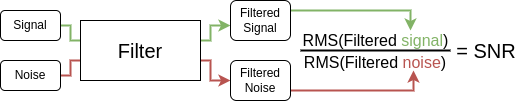
\includegraphics[width=1.0\columnwidth]{images/filter_process.png}
	\end{center}
	\caption{Illustration of testing of filters. Signal and noise are passed through the filter individually and the SNR is calculated for each filter.}
	\label{fig:filter_process}
\end{figure}

SNR by itself is not a valid metric for judging a filters performance in this scenario. The purpose of improving SNR is the assumption that force can be estimated more accurately from a signal that contains primarily the signal generated by muscle contraction. However, a filter may be able to attenuate the signal and noise in such a way that the SNR is very high, but the signal is attenuated to such a degree that it no longer resembles the original signal that was generated by the muscle contraction. An example of this can be seen in Figure~\ref{fig:good_snr_bad_integrity}. 

A measure to define how much the frequency spectrum has changed is the bandwidth. Typically the bandwidth of a signal is defined as the range of frequencies between two frequency points outside of which the signal is attenuated more than a specific threshold value \cite{bandwidth_definition}. This definition is not applicable to this problem as the frequencies that are 'present' in an sEMG signal are not necessarily consecutive. Therefore the bandwidth of an sEMG signal will be defined as the number of frequency components that are larger than the mean of the frequency spectrum. With this metric, a frequency spectrum such as the one seen in Figure~\ref{fig:good_snr_bad_integrity} will have a low bandwidth because most frequencies are below the mean.

\begin{figure}[h!t]
	\begin{center}
		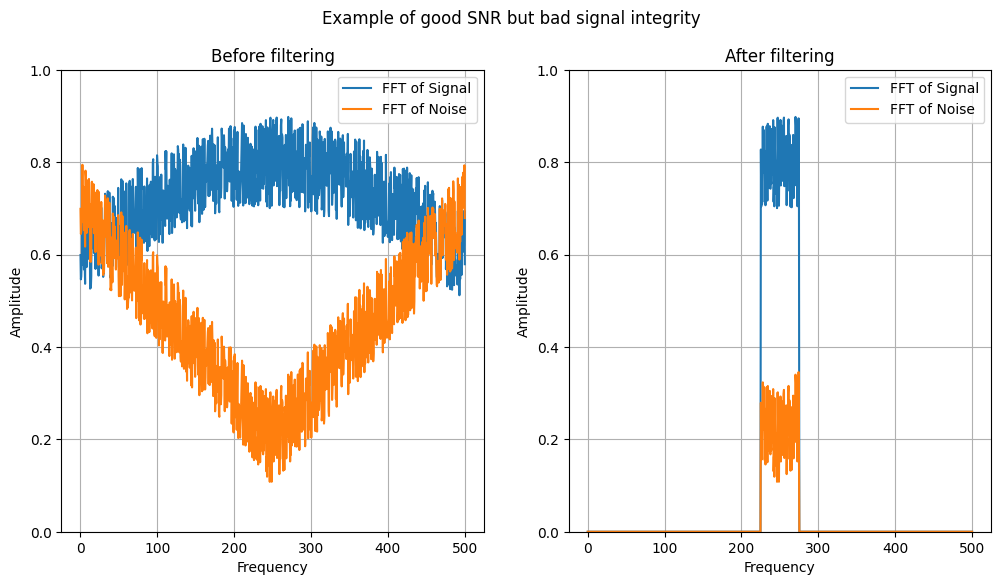
\includegraphics[width=1.0\columnwidth]{images/good_snr_bad_integrity.png}
	\end{center}
	\caption{Example of filtering that results in good SNR but bad bandwidth.}
	\label{fig:good_snr_bad_integrity}
\end{figure}


\subsection{Method}
\subsubsection{Static filter}
The theory from section \ref{section:standard_semg_processing} specifies the removal of DC frequencies, a notch filter at \SI{50}{Hz}, and a bandpass filter between \SI{20}{Hz} and \SI{300}{Hz}. Looking at the noise spectrum in Figure~\ref{fig:sEMG_fft_signalnoise_example} it can be seen that there also exist significant peaks at \SI{100}{Hz} and \SI{150}{Hz}. Therefore different static filters were tested with different amounts of notch filters. 

\begin{itemize}
    \item IIR Notch filters at \SI{50}{Hz}, \SI{100}{Hz}, \SI{150}{Hz}, \SI{200}{Hz}. All have a Q-factor of 10, are constructed as numerator/denominator pairs and applied using scipy's lfilter.
    \item The bandpass filter consists of a high-pass filter with an $f_{cut}$ of \SI{20}{Hz} and a lowpass filter with an $f_{cut}$ of \SI{300}{Hz}. Both filters are of length 5, are constructed as numerator/denominator pairs, and applied using scipy's lfilter.
\end{itemize}

The frequency response of these filters can be seen in Figure~\ref{fig:staticfilter_notches_frequencyresponse}. The resulting metrics can be seen in the chart \ref{fig:staticfilter_notches_barchart}.

\begin{figure}[h!t]
	\begin{center}
		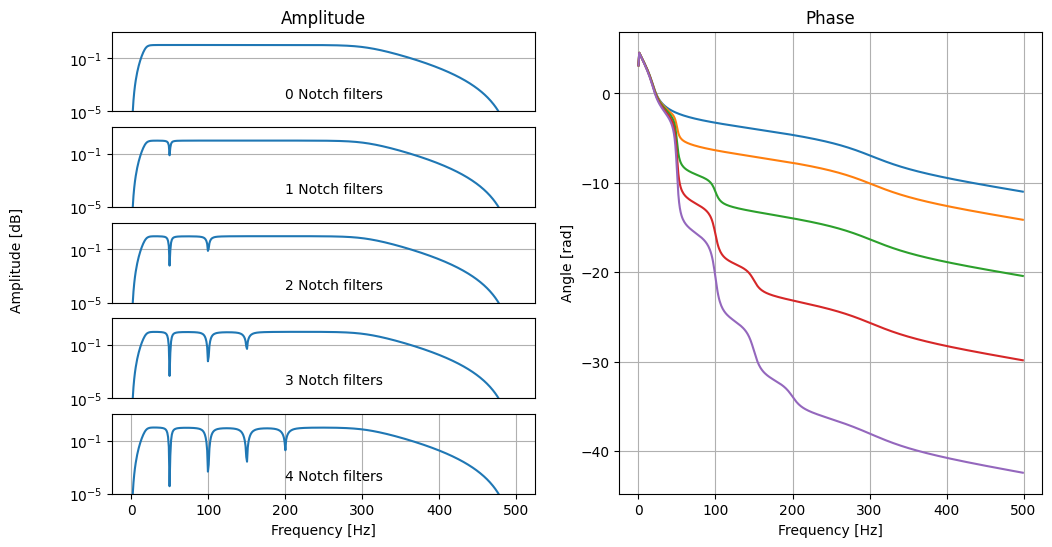
\includegraphics[width=1.0\columnwidth]{images/staticfilter_notches_frequencyresponse.png}
	\end{center}
	\caption{Frequency response of static filters with a different number of notch filters. The plots were created by determining the frequency responses of each individual filter (notches, low-pass, high-pass), then multiplying the amplitudes and adding the phase shifts. For the sake of illustration the amplitude graphs have been shifted vertically to clearly show the existence of notch filters in different lines, during simulations this shift was not present. }
	\label{fig:staticfilter_notches_frequencyresponse}
\end{figure}

\begin{figure}[h!t]
	\begin{center}
		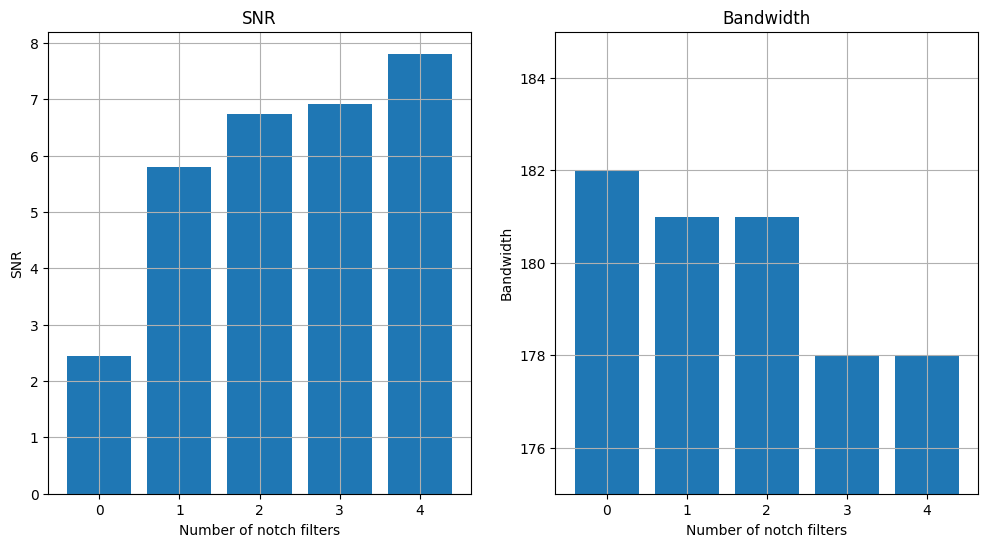
\includegraphics[width=1.0\columnwidth]{images/staticfilter_notches_barchart.png}
	\end{center}
	\caption{SNR and bandwidth of static filters with different numbers of Notch filters. Three notch filters were chosen for the measurement section (\ref{sec:measurements}) as the bandwidth seems to not depend very much on number of filters but in Figure~\ref{fig:sEMG_fft_signalnoise_example} the peak around \SI{200}{\hertz} is insignificant compared to other multiples of \SI{50}{\hertz}}
	\label{fig:staticfilter_notches_barchart}
\end{figure}


\subsubsection{Wiener filter}
As discussed in section \ref{sec:filters_theory} the Wiener filter coefficients are constructed from the cross-correlation vector between signal+noise ($d(n)$) and the noise ($v(n)$) and the auto-correlation of the noise as is presented in the Wiener-Hopf equation in Equation~\ref{eq:wiener_hopf} \cite{lecture_adaptive_filters_1}. 

\begin{equation}
    w_{opt} = R^{-1}P
    \label{eq:wiener_hopf}
\end{equation}

The number of Wiener filter coefficients have a strong influence on the performance of the filter as can be seen in Figure~\ref{fig:wiener_filter_length}. For the measurements section (\ref{sec:measurements}), a Wiener filter of length 500 was chosen as this is a middle ground for SNR and bandwidth.

\begin{figure}[h!t]
	\begin{center}
		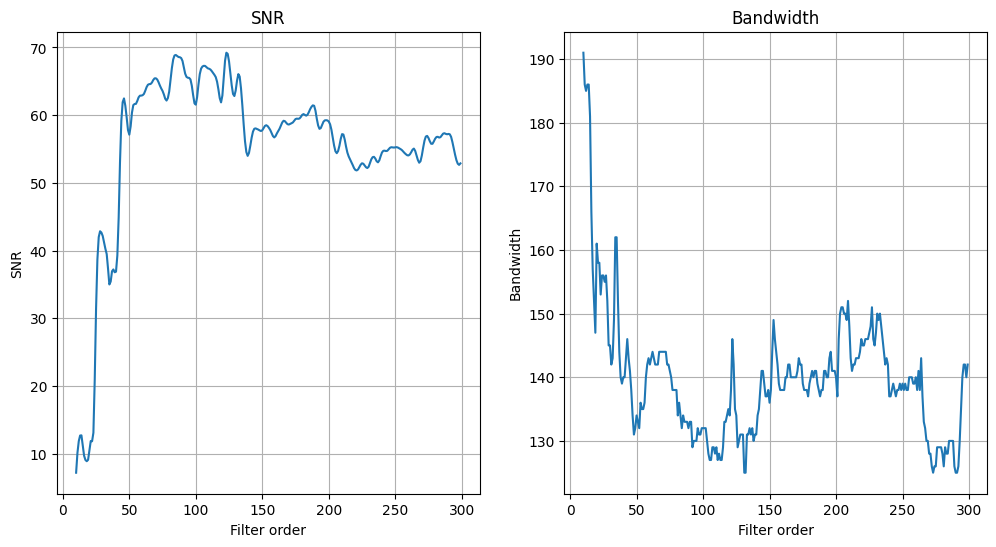
\includegraphics[width=1.0\columnwidth]{images/wiener_filter_length.png}
	\end{center}
	\caption{The effect of the number of Wiener filter coefficients on the SNR and bandwidth. To clarify the more general influence of filter length both plots were smoothed using a Savitzky-Golay filter with length of 71 and poly order of 3. It appears there is a clear peak in SNR at 650 filter terms but this corresponds to a low bandwidth. A filter length of 500 was chosen as this presents a good middle ground between SNR and bandwidth peak in the bandwidth. }
	\label{fig:wiener_filter_length}
\end{figure}

\begin{figure}[h!t]
	\begin{center}
		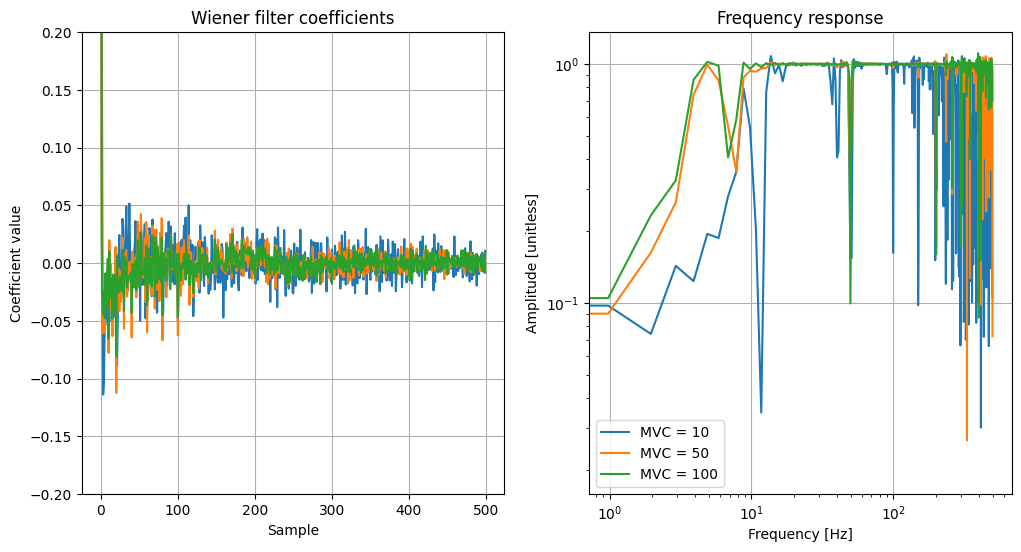
\includegraphics[width=1.0\columnwidth]{images/wiener_filter_response_mvc.png}
	\end{center}
	\caption{The frequency response of a Wiener filter at different levels of MVC. It can be seen that at a lower MVC the filter appears to have a very aggressive frequency response (seen by the large peaks at \SI{10}{\hertz} and higher frequencies) while at higher MVC this response is much less pronounced.}
	\label{fig:wiener_filter_response_mvc}
\end{figure}


\subsubsection{Adaptive filter}
The functioning of an LMS filter has been described in the theory section. An LMS filter has two properties that determine its behaviour: The filter length and the convergence coefficient. To determine the best combination of these parameters when applied to sEMG signals a range of different values was tested. The results can be found in Figure~\ref{fig:lms_filter_windowsize}. For the measurement section (\ref{sec:measurements}) an LMS filter with length 500 and convergence value of 0.1 will be used.

\begin{figure}[h!t]
	\begin{center}
		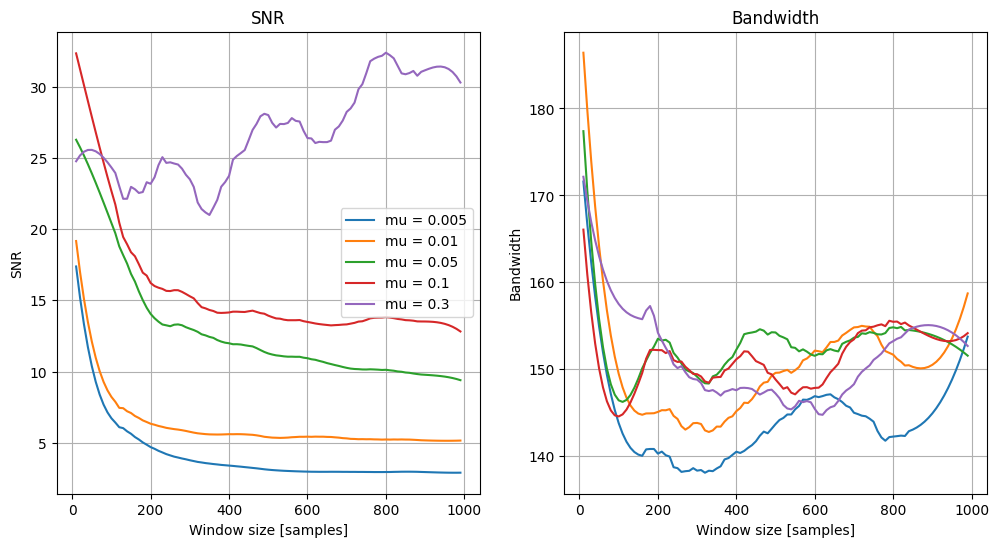
\includegraphics[width=1.0\columnwidth]{images/lms_filter_windowsize.png}
	\end{center}
	\caption{SNR and bandwidth of an adaptive LMS filter using different combinations of filter length and convergence value. It should be noted that each signal has been smoothed using a Savitzky-Golay filter with a window length of 31 and a polynomial order of 3. This is done to make the difference in performance between different convergence values clearer as without filtering the signals have a larger deviation that makes the lines unreadable. The SNR peaks with a filter length of around 600 samples and a convergence value of 0.3. However, in the bandwidth plot this convergence value corresponds to the worst option. A convergence value of 0.1 with a filter length of 500 was chosen as this yields a good middle ground between SNR and bandwidth}
	\label{fig:lms_filter_windowsize}
\end{figure}


\subsection{Results}
A property that might be of interest is each filters performance in different levels of Maximum Voluntary Contraction (MVC). This allows for insight into how well each filter functions in different levels of signal compared to the environment noise. This was realized by keeping the noise constant, but scaling the signal to different levels (from 1-\SI{100}{\percent}) to simulate different levels of MVC. The SNR of the filtered signal and filtered noise was divided by the reference SNR (SNR of input signal and input noise) to be able to draw a clear conclusion about the filters performance.

\begin{figure}[h!t]
	\begin{center}
		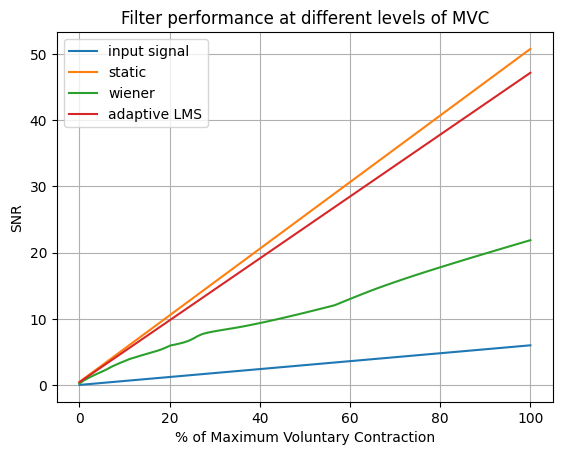
\includegraphics[width=0.7\columnwidth]{images/filter_snr_mvc.png}
	\end{center}
	\caption{The SNR of each filter for different levels of MVC. It can be seen that there is no relation between a filters performance and the degree of contraction for all the static filters. For the adaptive filter there is a strong negative relation between MVC and SNR. This will be further explored in the measurement section.}
	\label{fig:filter_snr_mvc}
\end{figure}

Again, the bandwidth was calculated for different filters and at different levels of MVC. The results can be seen in Figure~\ref{fig:filter_bw_mvc}.

\begin{figure}[h!t]
	\begin{center}
		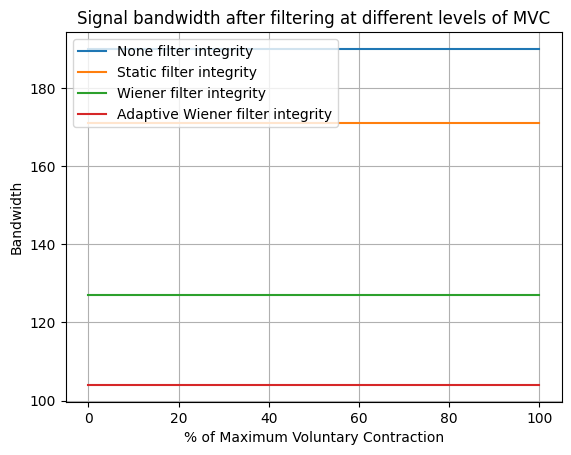
\includegraphics[width=0.7\columnwidth]{images/filter_bw_mvc.png}
	\end{center}
	\caption{The bandwidth of each filter for different levels of MVC. It can be seen that there is no relation between a filters performance and the degree of contraction. }
	\label{fig:filter_bw_mvc}
\end{figure}

For bandwidth holds that the metric is independent of degree of muscle contraction as seen in Figures~\ref{fig:filter_bw_mvc} and for SNR this holds except for the non-static adaptive LMS filter as seen in Figure~\ref{fig:filter_snr_mvc}
Figure~\ref{fig:filter_snr_mvc} shows that the best signal to noise ratio is achieved using a Wiener filter, but this filter also has the worst bandwidth performance as seen in Figure~\ref{fig:filter_bw_mvc}. 

\section{Envelope estimation}
\subsection{Comparison metrics}
There are two separate metrics that need to be measured when comparing envelope estimation techniques. The first one is how 'fast' a techniques is, and the second is how 'good' the technique is. The first metric gives information about how much the 'detected' signal lags behind the 'true' signal. The second metric is the quality of the envelope estimate when accounting for the lag.

The lag is detected by calculating the cross-correlation between the true signal and the envelope estimate. Cross-correlation is a metric that determines the similarity between two signals as a function of displacement of one signal relative to another \cite{wiki:cross_correlation}. Since the 'true' signal and the estimated signal are most similar when their displacement equals the lag, a detectable peak is formed in the cross correlation function. The left subplot in Figure~\ref{fig:envelope_estimation_method} displays a 'true' signal (measured force), and a simulated estimation of this signal (estimated force) that lags behind the true signal. The cross-correlation is also plotted that has a peak at \SI{100}{\milli\second}, which is the exact amount of lag between the two signals. The right subplot shows the two signals where the estimated signal has shifted to account for the lag. 

The error can be determined by subtracting the true signal from the estimated signal, and the root-mean-square-error can be calculated. 

\begin{figure}[h!t]
	\begin{center}
		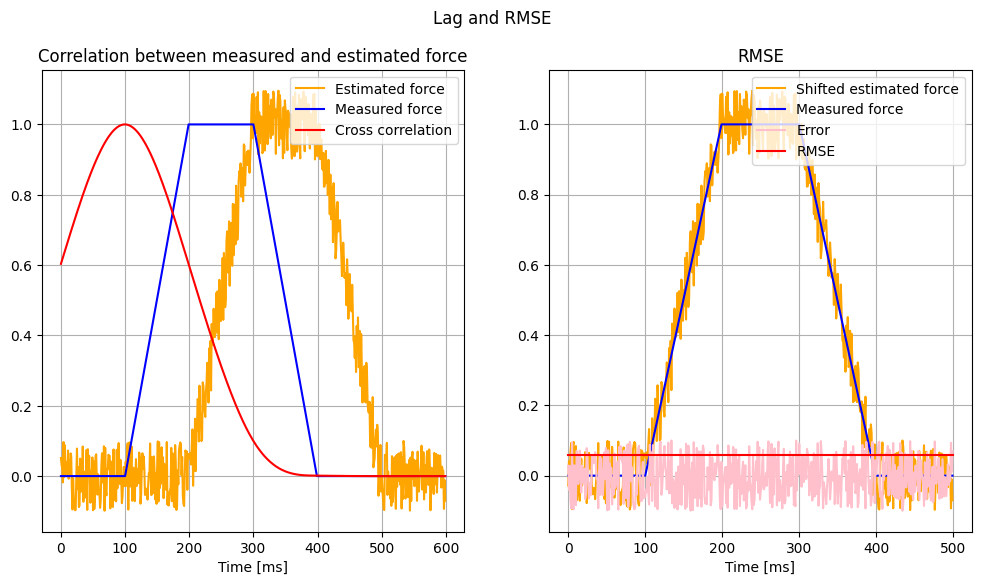
\includegraphics[width=1.0\columnwidth]{images/envelope_estimation_method.png}
	\end{center}
	\caption{Illustration of method for judging envelope estimation}
	\label{fig:envelope_estimation_method}
\end{figure}

An input signal was generated to be Gaussian white noise since it has signal properties close to that of an sEMG signal, and is multiplied with a modulation that can be seen in the left subplot of Figure~\ref{fig:envelope_detection}. The envelope detection techniques are applied onto the input signal and the results are plotted in the right subplot of Figure~\ref{fig:envelope_detection}.

\begin{figure}[h!t]
	\begin{center}
		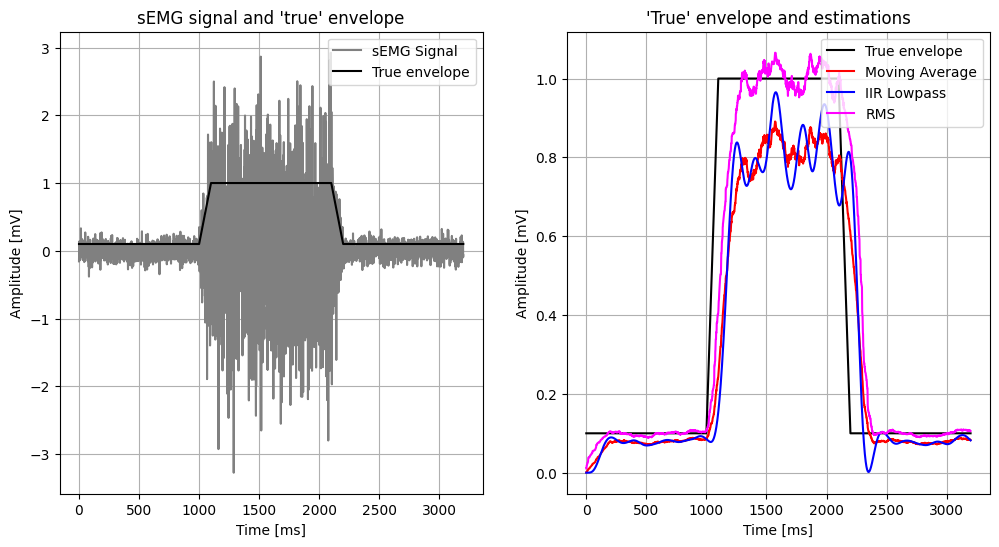
\includegraphics[width=1.0\columnwidth]{images/envelope_detection.png}
	\end{center}
	\caption{Left: Input signal and 'true' envelope'. Right: Envelope detection using different techniques to illustrate difference in behaviour}
	\label{fig:envelope_detection}
\end{figure}

\subsection{Method}
\subsubsection{IIR lowpass filter}
A Butterworth filter was used to construct an IIR lowpass filter. The performance of such a lowpass filter is defined by its $f_{cut}$ and the number of filter coefficients (or the filter order). It was empirically determined that the maximum frequency for switching between total relaxation and maximum voluntary contraction was around \SI{5}{\hertz} and thus the $f_{cut}$ was varied from \SI{1}{\hertz}-\SI{9}{\hertz}. The filter order was varied from 2-8 because the minimum possible filter order is 2 (a single filter coefficient provides no filtering, just scaling the signal with a constant), and a filter order >8 resulted in unstable behaviour. A plot of the frequency response of the IIR Butterworth filter can be seen in Figure~\ref{fig:iir_frequencyresponse_coefficients}. The filters are achieved as a numerator/denominator sequence. Since the purpose of this filter is real-time envelope detection, it was applied using scipy's lfilter since as that is causal forward-in-time filtering only.


\begin{figure}[h!t]
	\begin{center}
		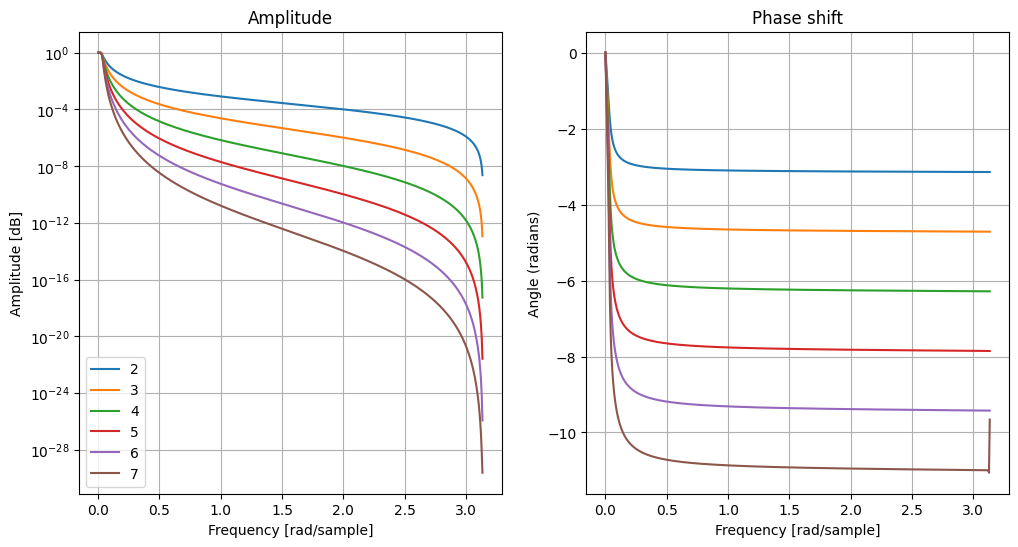
\includegraphics[width=1.0\columnwidth]{images/iir_frequencyresponse_coefficients.png}
	\end{center}
	\caption{Frequency response of IIR Butterworth filter of different order. The $f_{cut}$ was set to 5Hz.}
	\label{fig:iir_frequencyresponse_coefficients}
\end{figure}

\subsubsection{Moving average}
The moving average filter only depends on the length of the filter, Figure~\ref{fig:movingaverage_frequencyresponse_coefficients} depicts the frequency behaviour of the moving average filter of different lengths. The range of values that are tested is chosen arbitrarily, but large enough to cover general use cases.

\begin{figure}[h!t]
	\begin{center}
		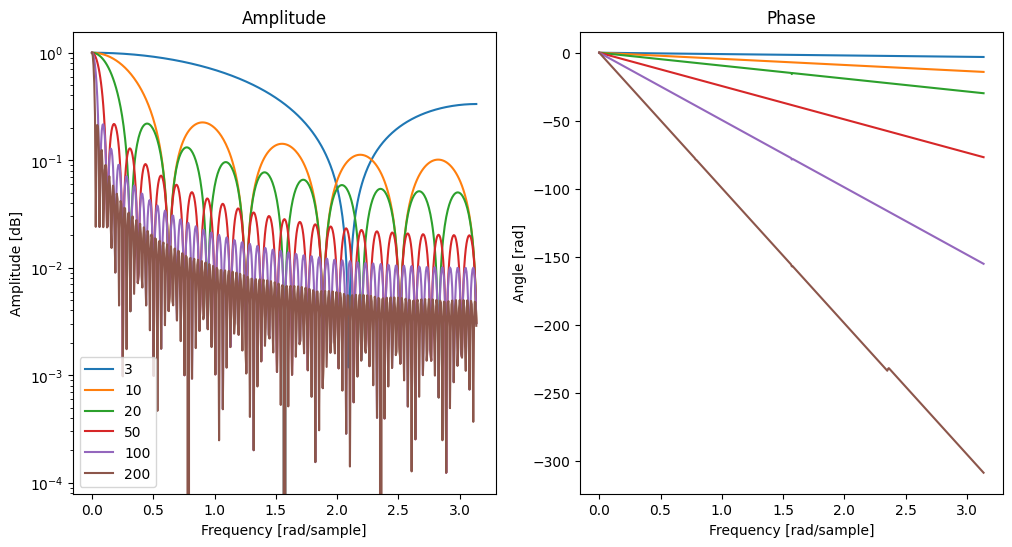
\includegraphics[width=1.0\columnwidth]{images/movingaverage_frequencyresponse_coefficients.png}
	\end{center}
	\caption{Frequency response of moving average filter of different lengths. The coefficients of the moving average filters are 1/length of filter.}
	\label{fig:movingaverage_frequencyresponse_coefficients}
\end{figure}

\subsubsection{Root mean square}
Similar to the moving average filter, the behaviour of the RMS filter is solely determined by the length of the filter. The same range of filter lengths was chosen as for the moving average filter so that the performance could be directly plotted against each other.

\subsection{Results}
To properly evaluate the performance of the envelope detection techniques each method has been tested individually across the range of variables that were described in the previous method section and plotted against the resulting lag and error. 

The graph describing the performance of the IIR Butterworth filter can be seen in Figure~\ref{fig:lagerror_iir}. The graph describing the performance of the moving average filter and the RMS filter can be seen in Figure~\ref{fig:lagerror_RMS_MA}.

\begin{figure}[h!t]
	\begin{center}
		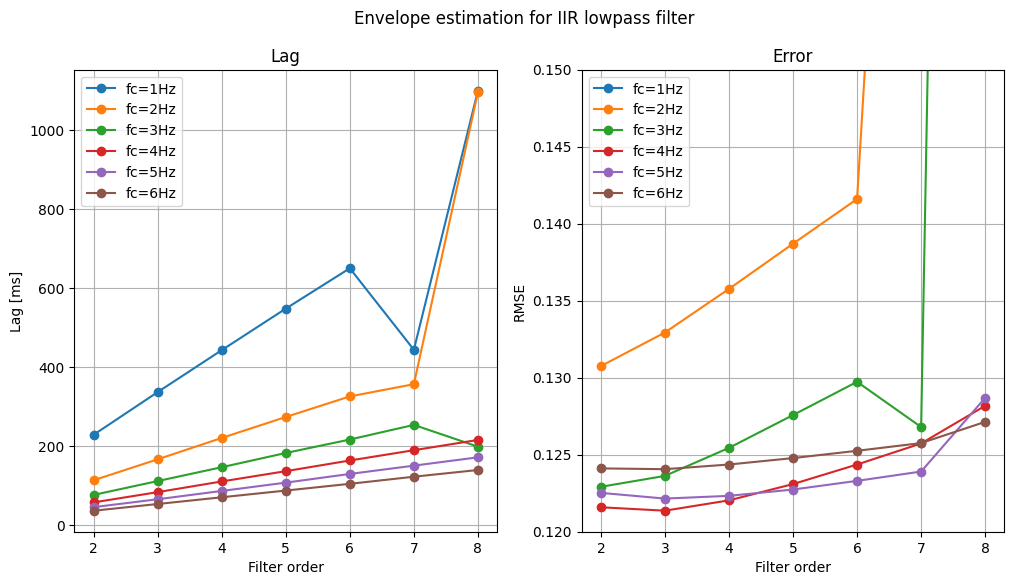
\includegraphics[width=1.0\columnwidth]{images/lagerror_iirfilter.png}
	\end{center}
	\caption{Lag and error of an IIR Butterworth filter for different cut-off frequencies and filter lengths. Note that filters with a lower $f_{cut}$ and high number of filter coefficients become unstable which can be seen in the error-graph for cut-off frequencies \SI{1}{\hertz}-\SI{3}{\hertz}. Additionally, the error in these graphs are all below 0.125. This is caused by the fact that the modulation is between 0 and 1, the error is <1 and the squared error is smaller still. So not the error value, but the \textit{relation between} error values of different methods is the truly useful information here.}
	\label{fig:lagerror_iir}
\end{figure}

\begin{figure}[h!t]
	\begin{center}
		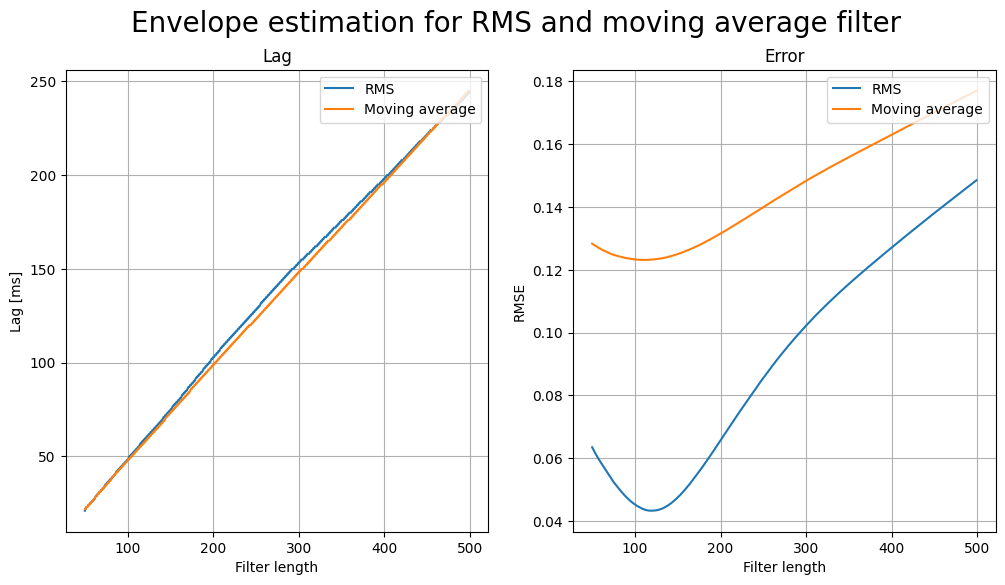
\includegraphics[width=1.0\columnwidth]{images/lagerror_rms_and_MA_filter.png}
	\end{center}
	\caption{Lag and error of RMS filter and moving average filter for different filter lengths}
	\label{fig:lagerror_RMS_MA}
\end{figure}

From Figure~\ref{fig:lagerror_iir} it can be seen that an IIR LP Butterworth filter of length 3 and $f_{cut}$ of \SI{4}{\hertz} results in the lowest error. A filter with $f_{cut}$ of \SI{6}{\hertz} has the lowest lag but this is only marginally less than a $f_{cut}$ of \SI{4}{\hertz}. For this reason an IIR LP Butterworth filter of length 3 and $f_{cut}$ of \SI{4}{\hertz} is used in the the measurement section (\ref{sec:measurements}).

From Figure~\ref{fig:lagerror_RMS_MA} it can be seen that moving average and RMS methods have similar lag, and the lag has a linear relation to the filter length. In the same figure it can also be seen that the error reaches a minimum at a filter length of 120. For this reason both the RMS and moving average method are applied with a filter length of 120.

\section{Force estimation}\label{section:force_estimation}
The measured sEMG signals from antagonistic muscles needs to be combined to form an estimate of the exerted force. Since this calculation is done in a consistent way throughout all measurements this section serves purely to provide some insight into the method of calculation.

The previous step of envelope estimation is used to get a measure of muscle activation. Since muscle activation leads to muscle contraction and exerted force around a joint is the difference between how much antagonistic contract \cite{human_robotics} it becomes possible to determine the force from sEMG. To correlate the difference in muscle contraction from antagonistic muscles (such as biceps and triceps) to the exerted force, the muscle contraction needs to be scaled. As previously mentioned, a linear relation between sEMG and force will be assumed \cite{adaptive_filter_dry_electrode} \cite{interpreting_muscle_function_from_emg}. In Figure~\ref{fig:force_simulation} it is shown how the exerted force is estimated from simulated bicep and triceps sEMG. 

\begin{figure}[h!t]
	\begin{center}
		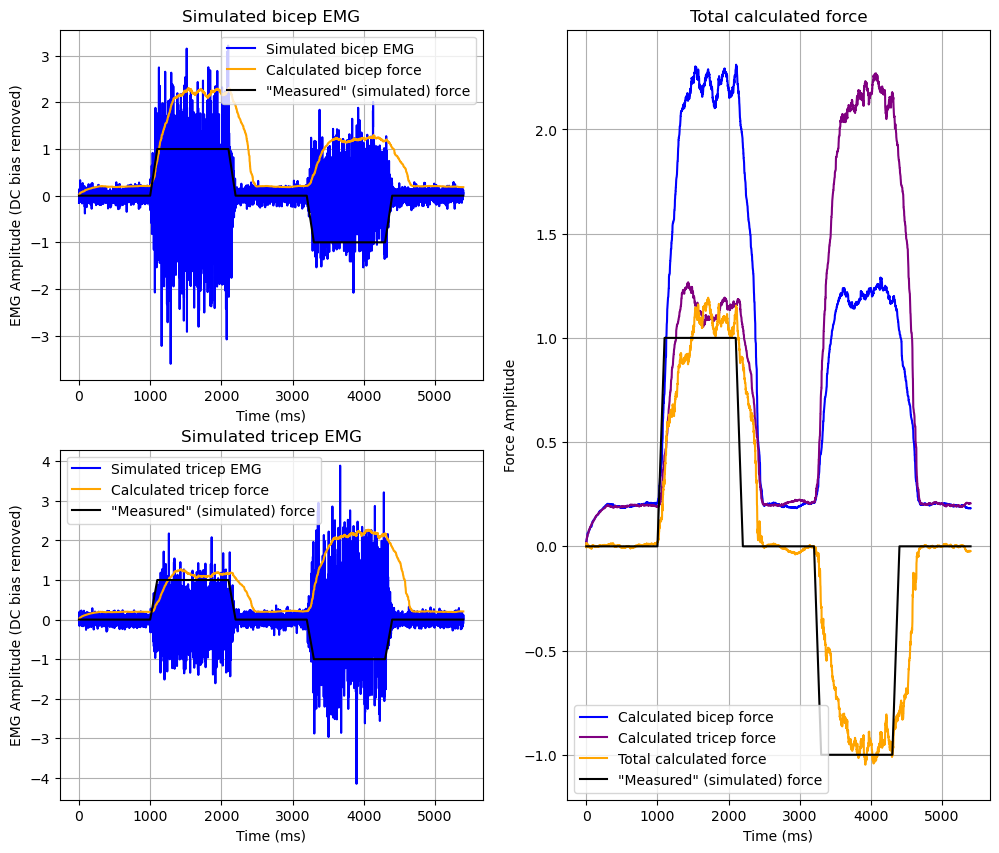
\includegraphics[width=1.0\columnwidth]{images/force_simulation.png}
	\end{center}
	\caption{Process of estimating force from simulated sEMG (random Gaussian noise). The bicep envelope is calculated at the top, notice how during downwards force exertion the bicep still activates but to a lesser degree than during upwards force exertion. The same holds for the triceps in the bottom figure. The subplot on the right shows the envelope of the bicep, triceps, the difference between these two (identical to estimated force assuming linear scaling with factor 1), and the 'measured' force .}
	\label{fig:force_simulation}
\end{figure}

\section{conclusion}
\chapter{Measurements}
This chapter aims to validate the accuracy of force estimation from sEMG after different processing techniques by comparing it to measured data. The goal is to measure sEMG from biceps and triceps, and record sEMG reference noise, and measure the estimated force using a load cell during an exercise of isometric contraction. The sEMG data is then processed using the different techniques that are discussed in the simulation chapter, and the final estimated force will be compared to the measured force. 

\section{Experimental setup}
The measurement setup consists of the following components:
\begin{itemize}
    \item Siemens Single Point Load Cell, 20kg Range, Compression Measure
    \item Keysight E3631A DC power supply at 2V to power the load cell
    \item TMSi Refa8-16e 16 channel amplifier
    \item Kendall H124SG Foam-Hydrogel ECG Electrodes 
\end{itemize}

The 16 channel amplifier performs unipolar measurements. This means that each electrode is connected to its own amplifier channel, and the measured values are compared to the value of a reference. The opposte of unipolar is bipolar which entails that the potential difference between two electrodes is amplified by a single amplifier channel \cite{tmsi_unipolar_bipolar}. 

The load cell has 4 relevant terminals. Two terminals are connected to the power supply to supply the load cell with power. The other two terminals are connected to the amplifier. The 'common' terminal of the power supply is connected to the 'Patient ground' on the amplifier.

Sets of two electrodes are placed on the subjects right bicep, right tricep, and left arm. The electrodes were placed following SENIAM guidelines \cite{seniam}. Two electrodes per set is chosen to essentially capture more data. Since each electrode in a set measures almost identical sEMG signal the signals from the electordes can be averaged to reduce any present noise. The electrodes on the left arm are used to record a reference noise. It is expected that this reference noise has an identical frequency spectrum as the noise present in the sEMG signal since it is recorded at the same time, approximately same place, using the same amplifier, and can therefore be used in some of the presented filtering techniques. The reference signal is recorded using a TMSi provided armband that was wetted and connected to 'Patient ground' on the amplifier. A total measurement setup diagram is shown in figure \ref{fig:measurement_setup_diagram}.

\begin{figure}[h!t]
	\begin{center}
		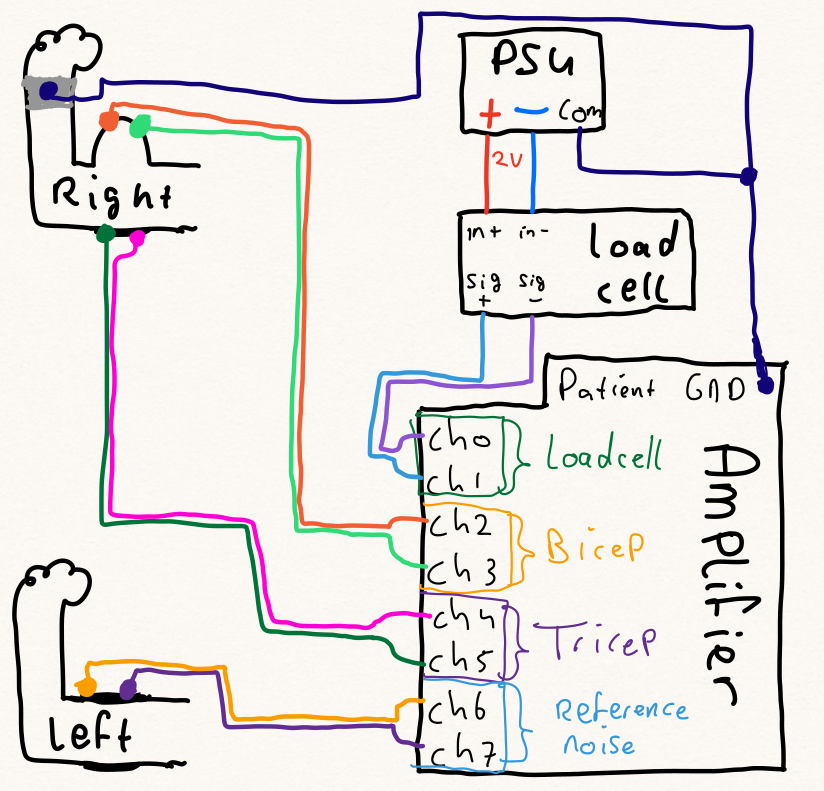
\includegraphics[width=1.0\columnwidth]{images/measurement_setup_diagram.png}
	\end{center}
	\caption{Diagram of the measurement setup}
	\label{fig:measurement_setup_diagram}
\end{figure}

\textcolor{red}{Todo: insert picture of holding load cell handle}

A total of four signal sets were recorded. Two measurements of applying force to the load cell at a sampling rate of \SI{1000}{\hertz} and \SI{20000}{\hertz}, and two accompanying load cell calibration measurements where an object with known weight was attached to the load cell at the sampling frequencies.

The applied force followed the following pattern:
\begin{itemize}
    \item Slowly pulling the handle upwards followed by a slow pushing the handle downwards. Repeated three times
    \item Slowly pull the load-cell upwards followed by returning to a neutral position. Repeated three times
    \item Slowly push the load-cell downwards followed by returning to a neutral position. Repeated three times
    \item Quickly pull the handle upwards followed by a quick push of the handle downwards. Repeated three times
\end{itemize}

\section{Measurement data}


\begin{figure}[h!t]
	\begin{center}
		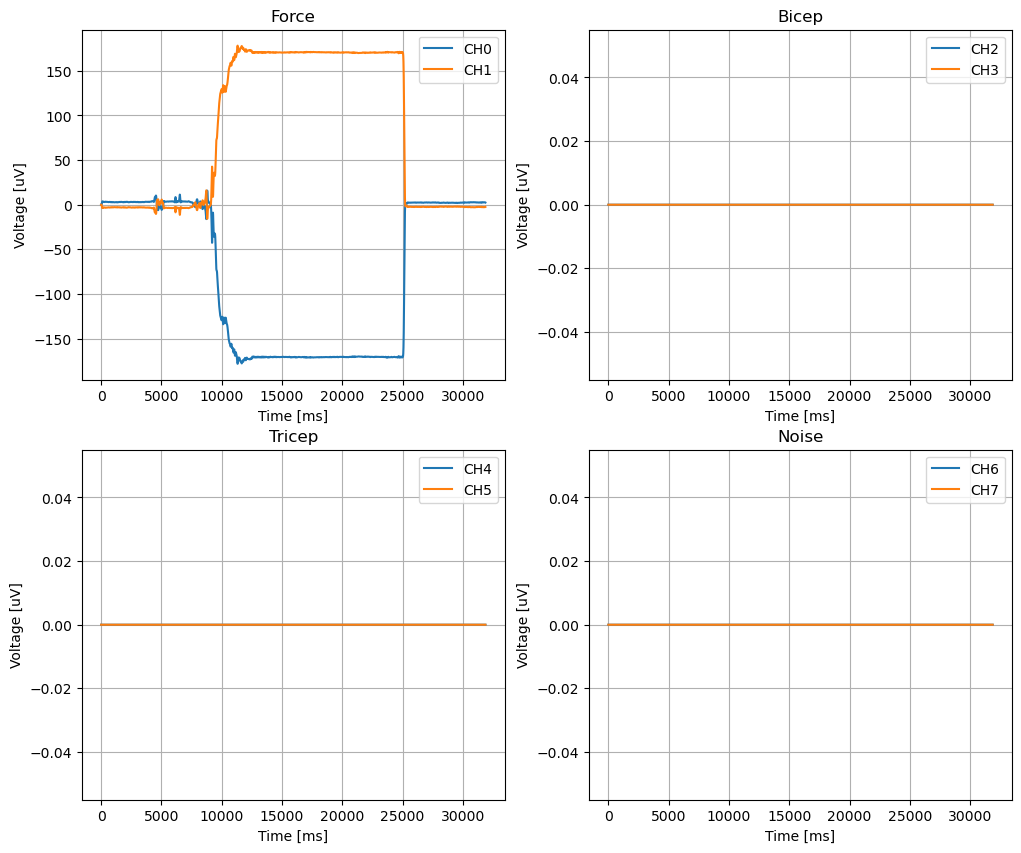
\includegraphics[width=1.0\columnwidth]{images/measurement_calibratie2_1k.png}
	\end{center}
	\caption{Calibration measurements at \SI{1}{\kilo\hertz} sampling rate. The force channels have been lowpassed with a cut-off frequency of 10 Hz to remove large \SI{50}{\hertz} noise component. The offset was determined to be \SI{2.5}{\micro\volt}. The weight op the object was \SI{1681}{\gram} which corresponds to \SI{167.5}{\micro\volt}}.
	\label{fig:calibration_1k}
\end{figure}

\begin{figure}[h!t]
	\begin{center}
		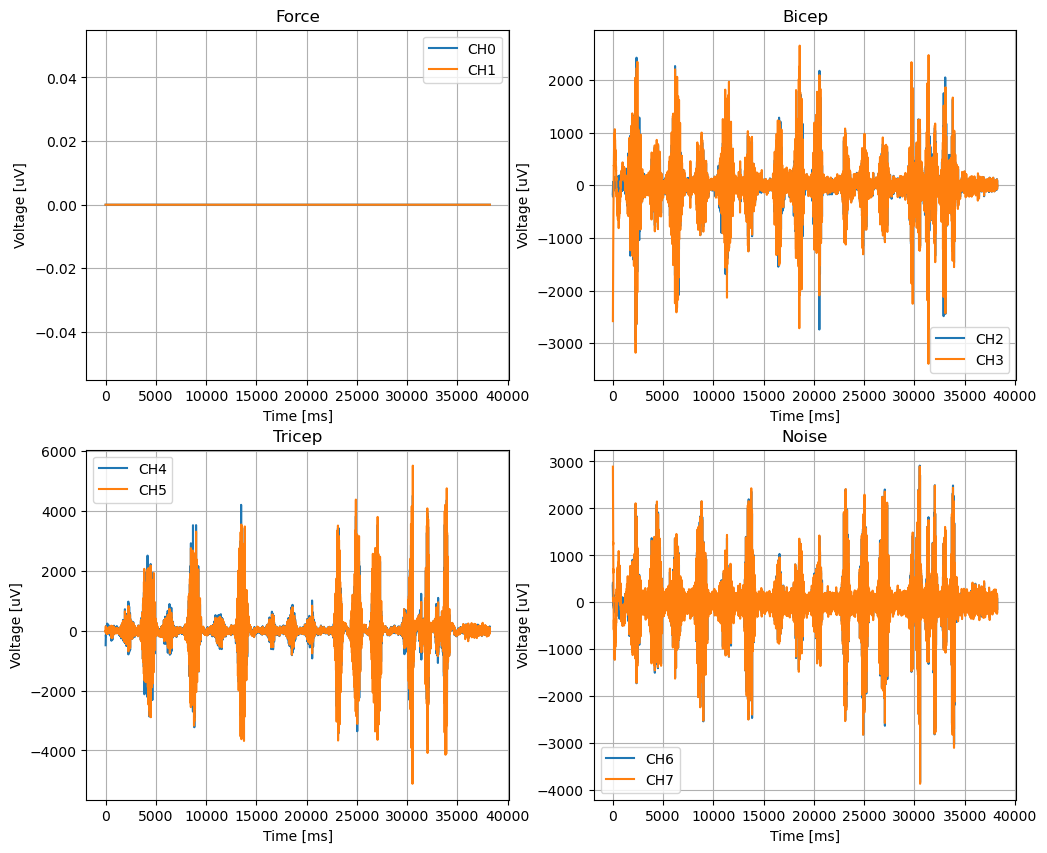
\includegraphics[width=1.0\columnwidth]{images/measurement_meting2_1k.png}
	\end{center}
	\caption{Force measurements at \SI{1}{\kilo\hertz} sampling rate}
	\label{fig:measurement_1k}
\end{figure}

The calibration process required measuring the steady-state value to determine the offset. To relate the measured values to the applied force, an object of known weight was attached to the load cell. These processes can be seen in figure \ref{fig:calibration_1k}. The measured force is approximately 10x the measured signal ($1681g / 167.5 uV = 10.03$).

Due to unknown reasons the amplifier was not able to capture both sEMG signals and the load cell signal at the same time which can be seen in figure \ref{fig:measurement_1k}. The load cell could be measured, but when attaching the the reference armband that the subject was wearing to 'Patient ground' on the amplifier the measured load cell signal was promptly nullified. Attaching the reference armband is required to measure sEMG signals, but connecting this armband makes it impossible to capture load cell information.

\section{Measurement processing result}
Force is estimation, no way to compare it to actual force. Make relative comments.

\begin{figure}[h!t]
	\begin{center}
		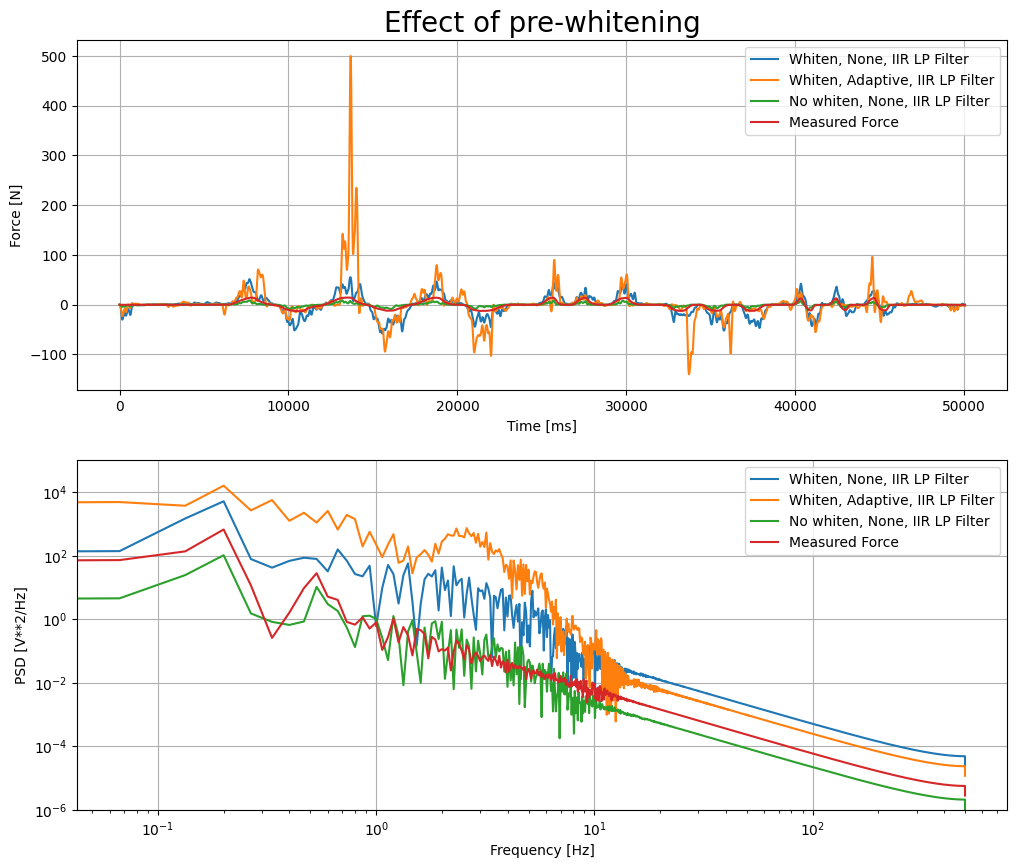
\includegraphics[width=1.0\columnwidth]{images/measurement_prewhitening.png}
	\end{center}
	\caption{Prewhitening}
	\label{fig:result_prewhitening}
\end{figure}

\begin{figure}[h!t]
	\begin{center}
		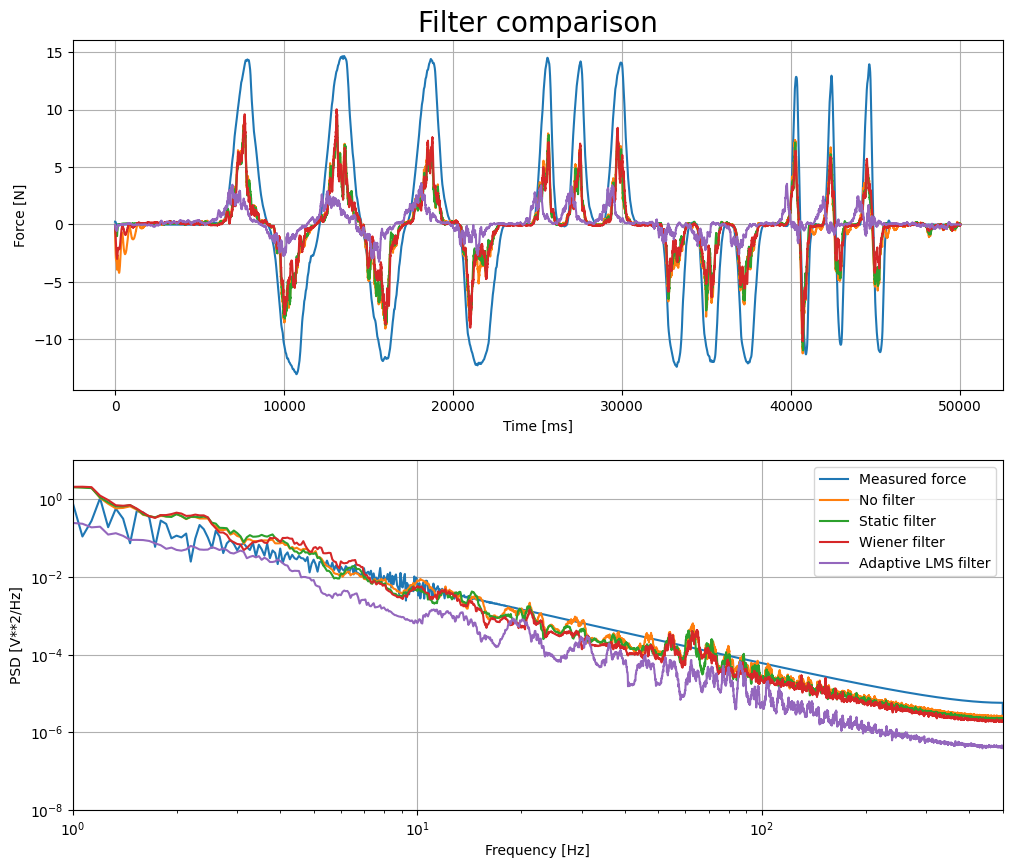
\includegraphics[width=1.0\columnwidth]{images/measurement_filtering.png}
	\end{center}
	\caption{Filtering}
	\label{fig:result_filtering}
\end{figure}
\begin{figure}[h!t]
	\begin{center}
		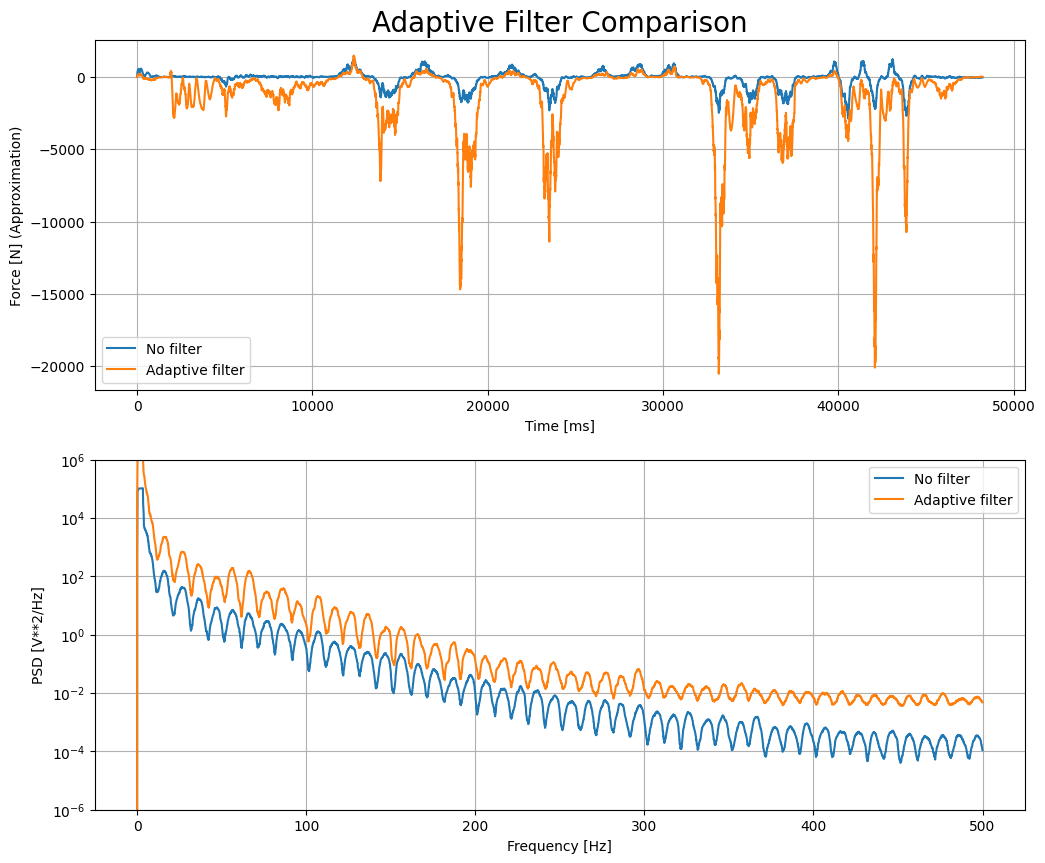
\includegraphics[width=1.0\columnwidth]{images/measurement_adaptive_filtering.png}
	\end{center}
	\caption{Adaptive filteirng}
	\label{fig:result_adaptive_filtering}
\end{figure}

\begin{figure}[h!t]
	\begin{center}
		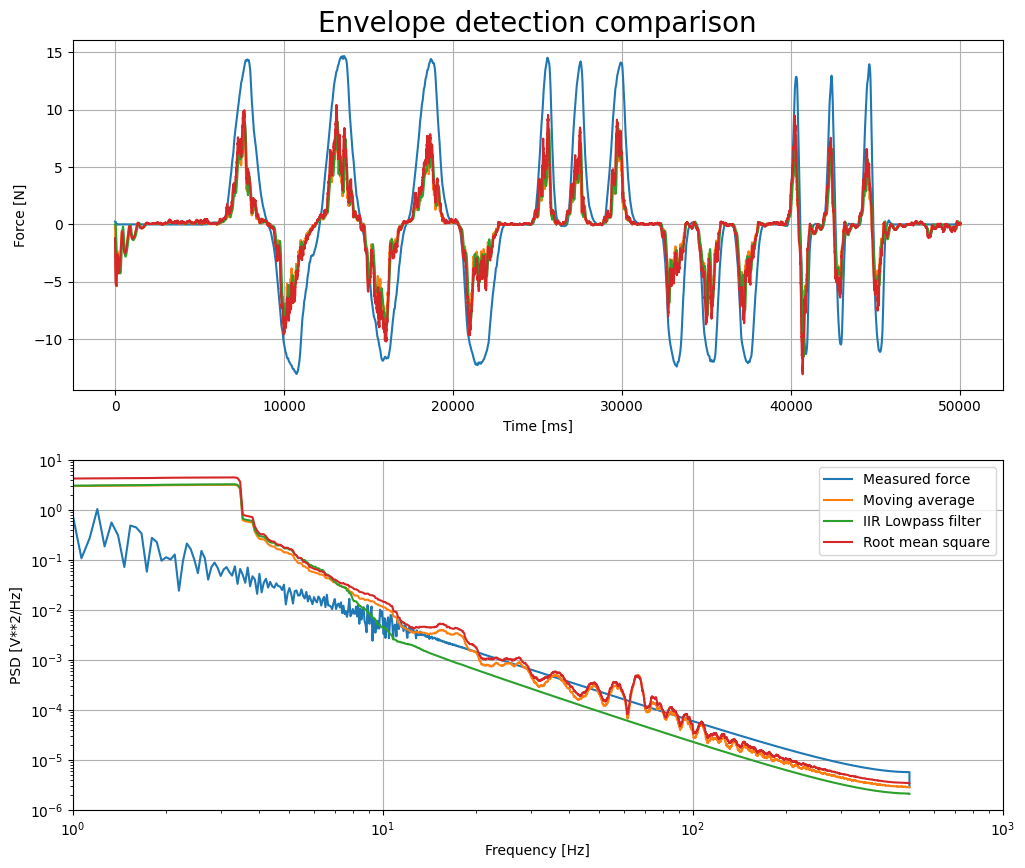
\includegraphics[width=1.0\columnwidth]{images/measurement_envelopes.png}
	\end{center}
	\caption{Envelopes}
	\label{fig:result_envelopes}
\end{figure}

pre-whiten plot
- no filter
- moving average envelope
- frequency spectrum is from 10-25s
=> delay

filter plot
- no prewhitening
- moving average envelope
- frequency spectrum is from 10-25s
- frequency plot is smoothened, moving average, n=50

adaptive filter plot
- no prewhitening
- moving average envelope
- frequency spectrum is from 10-25s
- frequency plot is smoothened, moving average, n=50
=> amplification 

envelopes
- no prewhitening
- moving average envelope
- frequency spectrum is from 10-25s
- frequency plot is smoothened, moving average, n=50
=> weird IIR lowpass filter behaviour


\section{Conclusion}
Draw numeric conclusion from data, in which situations is which filter how much better?
\chapter{Discussion and conclusion}
\section{Discussion}
The research question presented in the introduction states the goal of finding the best combination of whitening, filtering, and envelope detection to estimate force from sEMG. 

From the measurement results presented in figure \ref{fig:result_all_lagerrorscaling} the conclusion can be drawn that a processing chain consisting of no pre-whitening, no filtering, and infinite impulse response butterworth lowpass filter for envelope detection yields the best accuracy for force estimating. It has the lowest error rate of all techniques and introduces no lag.

This indicates that improving the signal to noise ratio of an sEMG signal does not result in a better estimation of the applied force. It should be noted that these conclusions are drawn from a single measurement at a single location and thus may yield different results in different environments. 

Another interesting observation can be made from the Lag comparison subplot in figure \ref{fig:result_all_lagerrorscaling}: only signal processing chains that use whitening appear to introduce lag. This could be caused by the phase delay that is introduced by the whitening filter. If the filter were to have a linear phase then all frequencies would be equally delayed resulting in a constant group delay. If this filter did not have linear phase but instead introduces a stronger phase delay in higher frequencies, then the total delay would become more apparent when amplifying these higher frequencies \cite{phase_delay_frequencies}. The amplification of higher frequencies does happen in the whitening filter as can be seen in the simulation in \ref{fig:whitening_simulation}, and the time domain plot shows signs of introduction of delay in the filtered signal which can stem from making higher frequencies with more phase delay more prominent. In the simulations the phase of the whitening filter was set to the phase of the input signal ('source' of filter). In the appendix are the results of constructing the whitening filter using zero-phase, linear-phase, and negative input signal phase \ref{fig:result_whitening_linearphase} \ref{fig:result_whitening_negative_sourcephase}\ref{fig:result_whitening_sourcephase}\ref{fig:result_whitening_zerophase}. Intuitively it would be expected that using negative source phase would counteract this introduced delay, but as can be seen in appendix figure \ref{fig:result_whitening_negative_sourcephase} this does not appear to be the case.

A reason why other processing steps do not seem to introduce delay when not paired with whitening could be that lag is calculated using the cross-correlation between the measured force and the estimated force. If the estimated force accurately follows the measured force, there would exist a clear peak in the cross-correlation which indicates the lag.




=> Other signals noise is larger than lag 


=> Combination of adaptive + whitening == very very bad
- instability of IIR filter

=> Beantwoorden van onderzoeksvraag

=> We make this conclusion but that only holds under these cirumstances

describe what your results mean and how they are an important contribution to the research field.

- short signal sample of MVC and noise
- no load cell measurement


What does it all mean?
◼ What hypotheses were proved or disproved?
◼ What did we learn?
◼ Why is it important (enough to report)?
\section{Conclusion}
In this report a complete signal processing chain for sEMG signals was presented. Within each step in this processing chain various processing techniques were discussed and tested to illustrate their behaviour and performance when applied to sEMG signals. 



Summarize your key findings. Include important conclusions that can be drawn and further implications for the field. Discuss benefits or shortcomings of your work and suggest future areas for research.

High-level conclusion that was not previously mentioned (The adaptive filter is better in X situation but at the cost of Y)

Summarize general trends in the data without comment, bias, or interpretation.
◼ Should add a new, higher level of analysis, and explicitly indicate the importance
of the work
◼ Do not repeat the Results section, unless special emphasis is needed
◼ Conclusions are not a summary of the work!

=> Samenvatting discussie met alleen de belangrijkste punten

\section{Recommendations}
Further research, suggestions for better results


% Appendix starts here
% change file name for better descriptive names, but start with apx-
\appendix
\chapter{Appendix 1} \label{app:whitening}

\begin{figure}[h!t]
	\begin{center}
		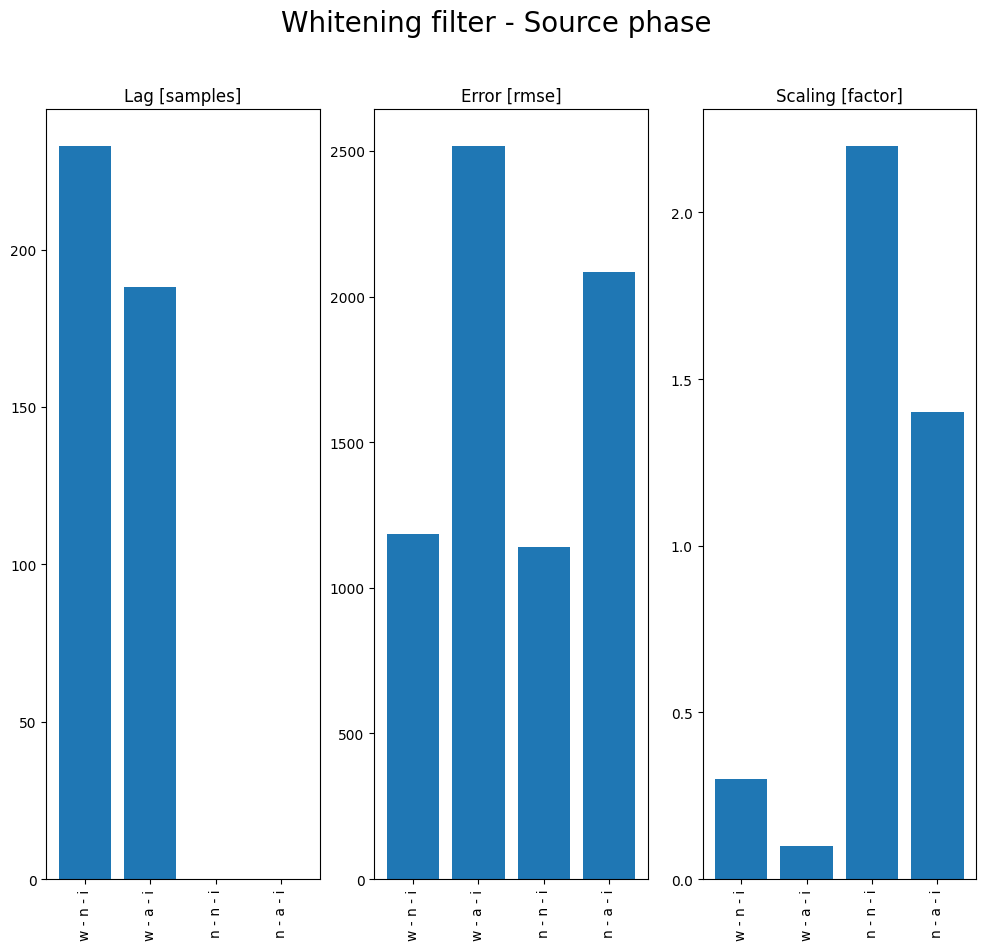
\includegraphics[width=1.0\columnwidth]{images/result_whitening_sourcephase.png}
	\end{center}
	\caption{Lag, error, and scaling of different filtering and envelope techniques with whitening applied. The whitening filter is constructed from the desired frequency amplitude response and a phase. The frequency response is determined as described in the simulation section \ref{sec:whitening}, and the phase is set to the phase of the input signal that was used to construct the whitening filter. }
	\label{fig:result_whitening_sourcephase}
\end{figure}

\begin{figure}[h!t]
	\begin{center}
		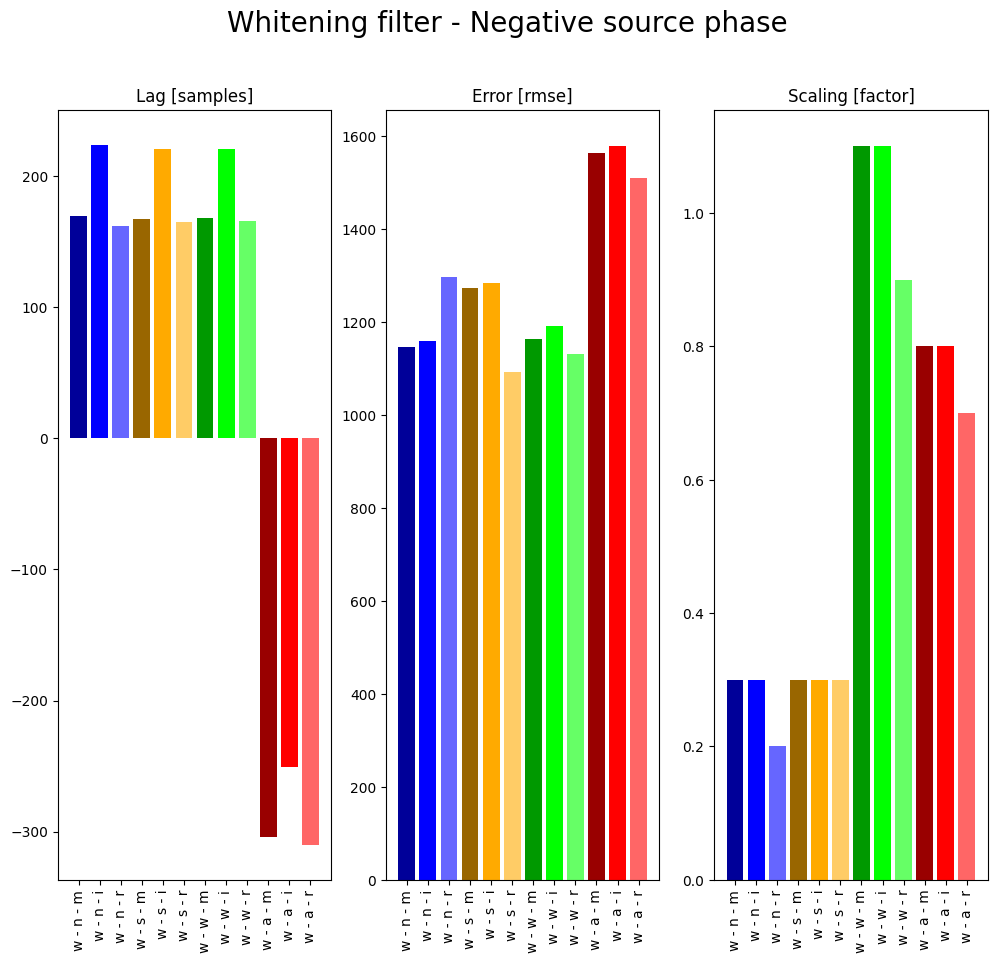
\includegraphics[width=1.0\columnwidth]{images/result_whitening_negative_sourcephase.png}
	\end{center}
	\caption{Lag, error, and scaling of different filtering and envelope techniques with whitening applied. The whitening filter is constructed from the desired frequency amplitude response and a phase. The frequency response is determined as described in the simulation section \ref{sec:whitening}, and the phase is set to the negative phase of the input signal that was used to construct the whitening filter. }
	\label{fig:result_whitening_negative_sourcephase}
\end{figure}

\begin{figure}[h!t]
	\begin{center}
		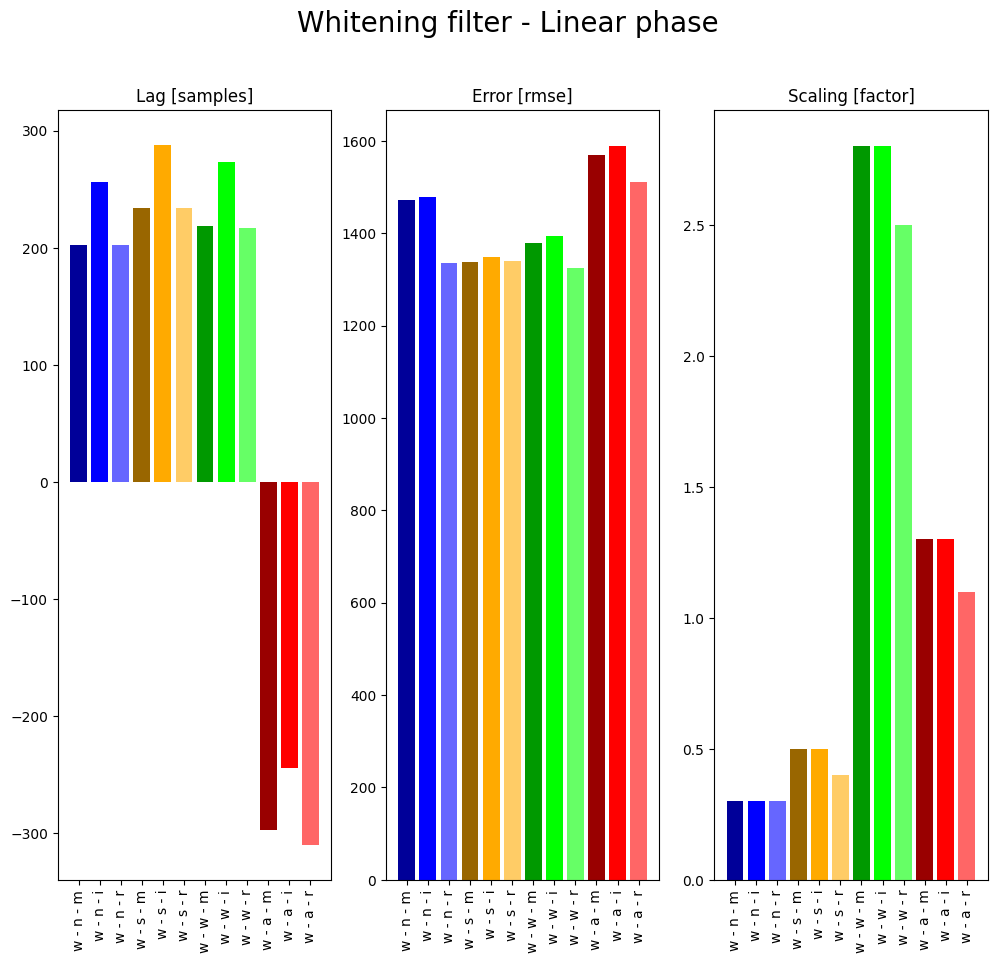
\includegraphics[width=1.0\columnwidth]{images/result_whitening_linearphase.png}
	\end{center}
	\caption{Lag, error, and scaling of different filtering and envelope techniques with whitening applied. The whitening filter is constructed from the desired frequency amplitude response and a phase. The frequency response is determined as described in the simulation section \ref{sec:whitening}, and the phase is set to linear phase. }
	\label{fig:result_whitening_linearphase}
\end{figure}

\begin{figure}[h!t]
	\begin{center}
		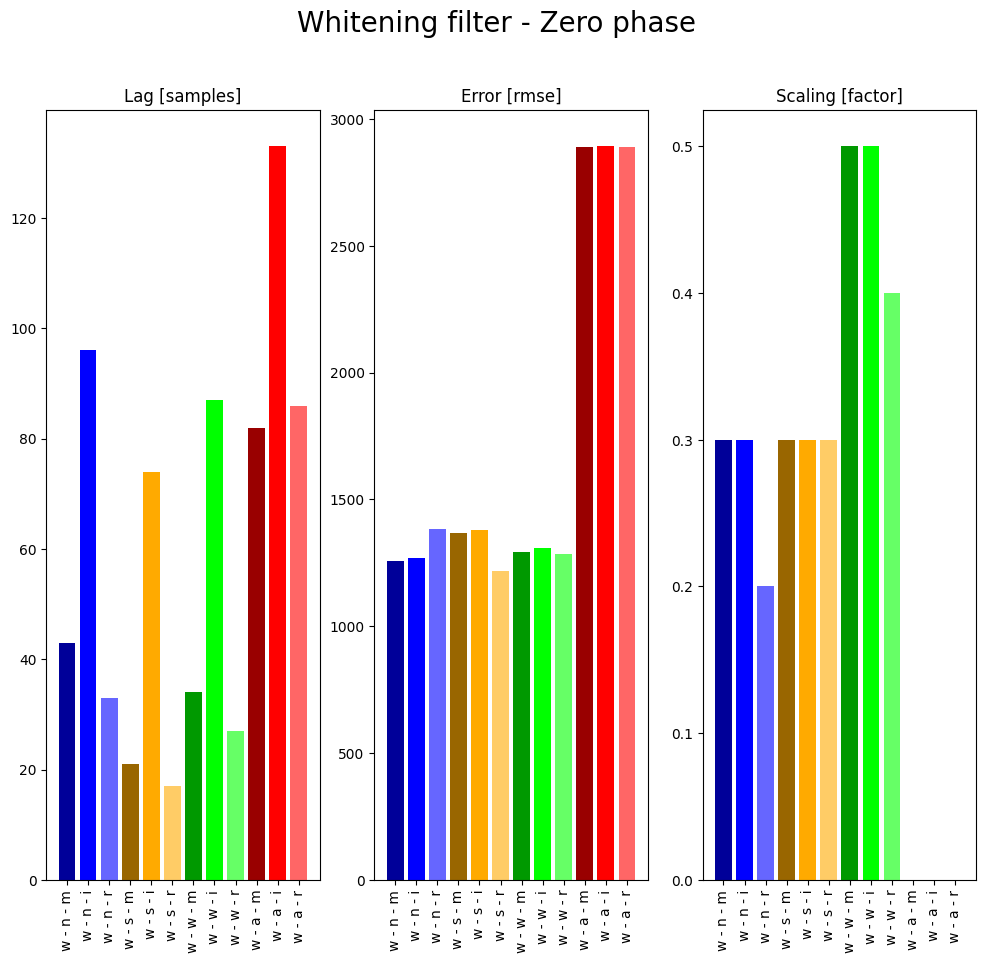
\includegraphics[width=1.0\columnwidth]{images/result_whitening_zerophase.png}
	\end{center}
	\caption{Lag, error, and scaling of different filtering and envelope techniques with whitening applied. The whitening filter is constructed from the desired frequency amplitude response and a phase. The frequency response is determined as described in the simulation section \ref{sec:whitening}, and the phase is set to zero phase. }
	\label{fig:result_whitening_zerophase}
\end{figure}

% Bibliography starts here
\backmatter

% Generate bibliography
\fancyhead[LO]{Bibliography}
%\bibliographystyle{include/files/RaM-bibtex}
\bibliographystyle{ieeetr}
\label{ch:bib} %label to refer to
\bibliography{bibliography} 

\end{document}

